\openepigraph{Memory... is the diary that we all carry about with us.}{---Oscar Wilde}

\section{Excel Tips}

This document gives a brief introduction to using excel for data analysis. The guide covers basic excel operation, formula use, and pivot tables. Many first time users will find aspects of excel confusing, this guide is intended to give you enough basic knowledge to get you started. There are extensive help guides published on the internet, and if you find yourself confronted with a problem that is not discussed here you will often find valuable help by searching Google for the answer. If you have suggestions for excel tips that should be included in this document please let your lab instructor know.

\subsection{What is Excel?}

Excel is a spreadsheet tool. It allows you to organize and analyze data that are stored in column and row format. Excel is extremely powerful. With enough know-how almost all of the data analysis that statistics programs like SPSS are built for, can be accomplished directly in Excel. 


\subsection{What is Excel used for in this course?}


You can use excel (or another spreadsheet program) to:


\begin{itemize} 

\item Store your data, 

\item to perform basic analysis of your data (e.g., getting averages and standard deviations, computing correlations etc.), and 

\item to create figures, graphs, and tables to present your data.
\end{itemize}


\section{Using Excel}

\subsection{The excel window}
 
Excel is a spreadsheet that contains different rows (the numbers), and different columns (the letters).
The individual cells can be used to hold data in the form of numbers or letters, to analyze data, and to report data using tables and figures.

\begin{figure}
      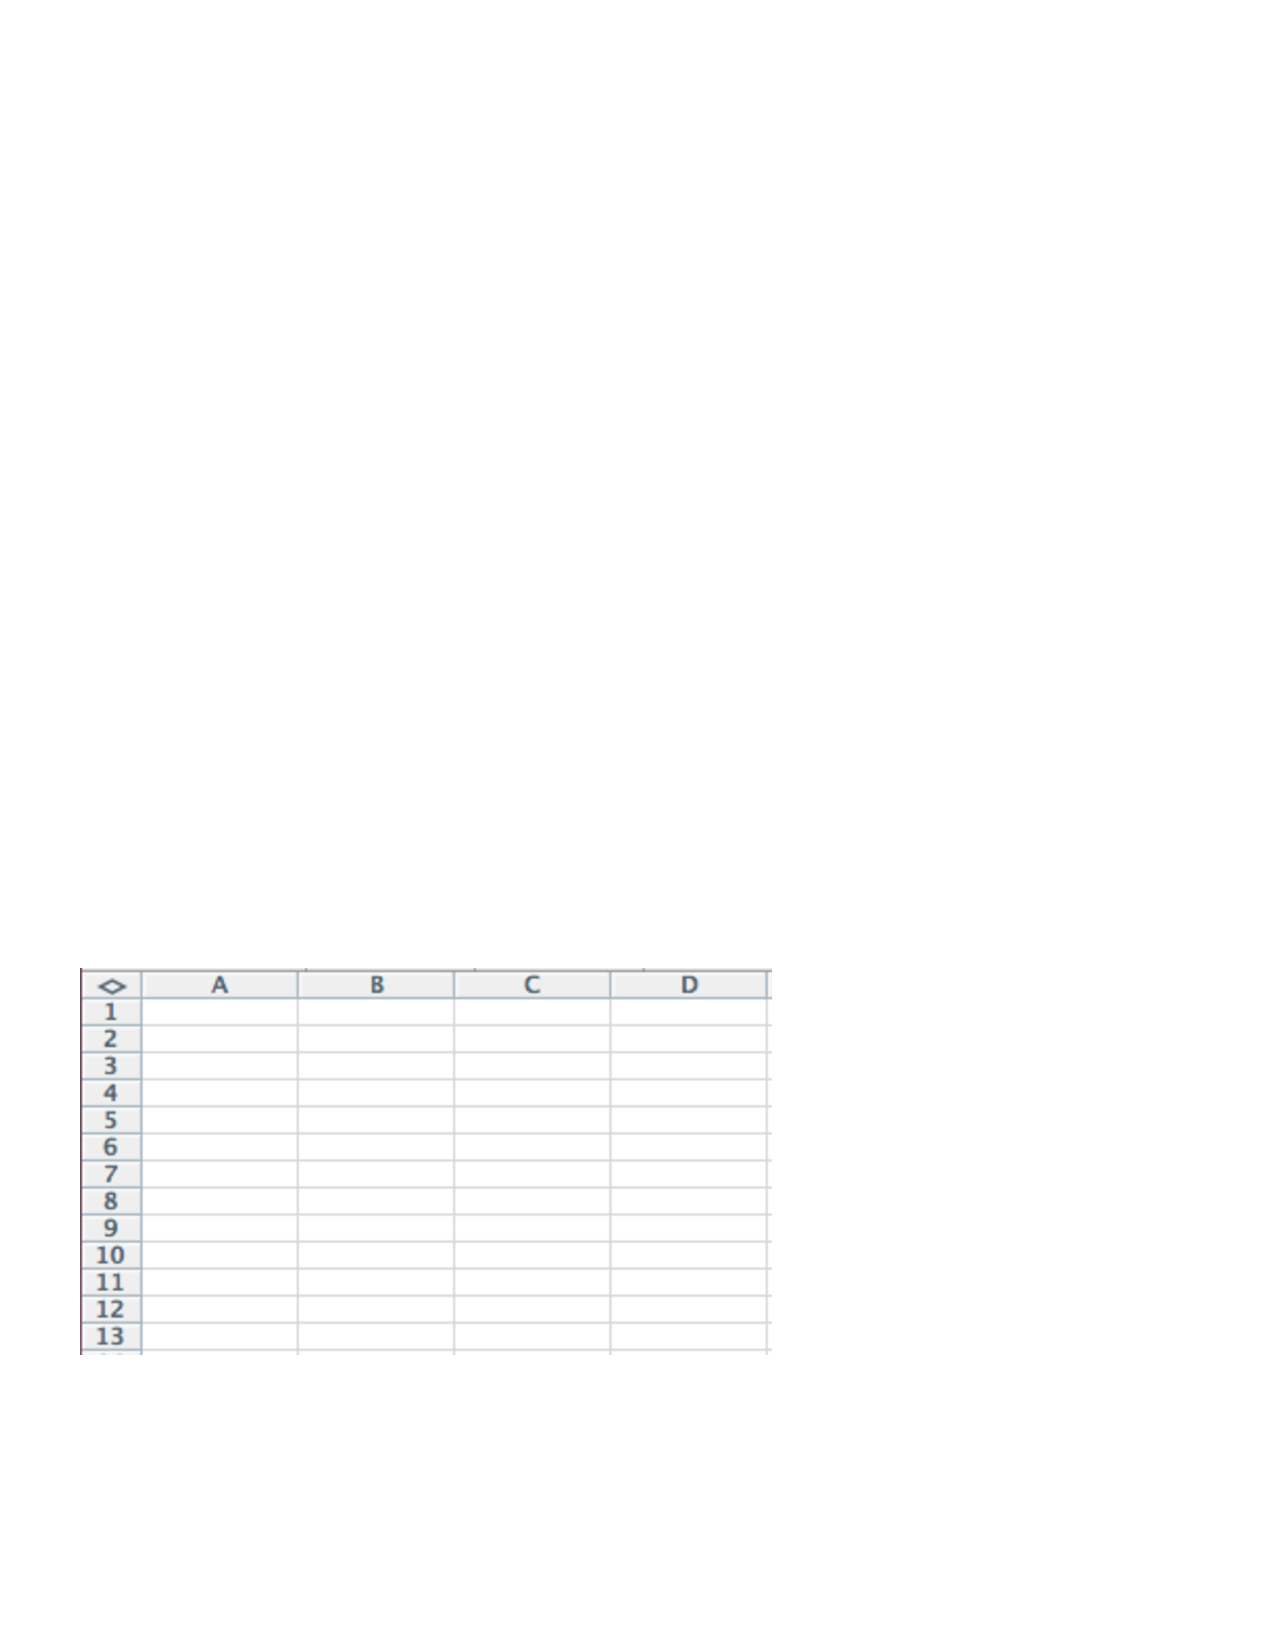
\includegraphics[width=.7\linewidth]{LabmanualFigures/Excel1.pdf}
      \caption{The excel window}
      \label{fig:excelwindow}
\end{figure}

\subsection{Inputting data}

Type or paste individual numbers or letters into individual cells, and then press return.

\begin{figure}
      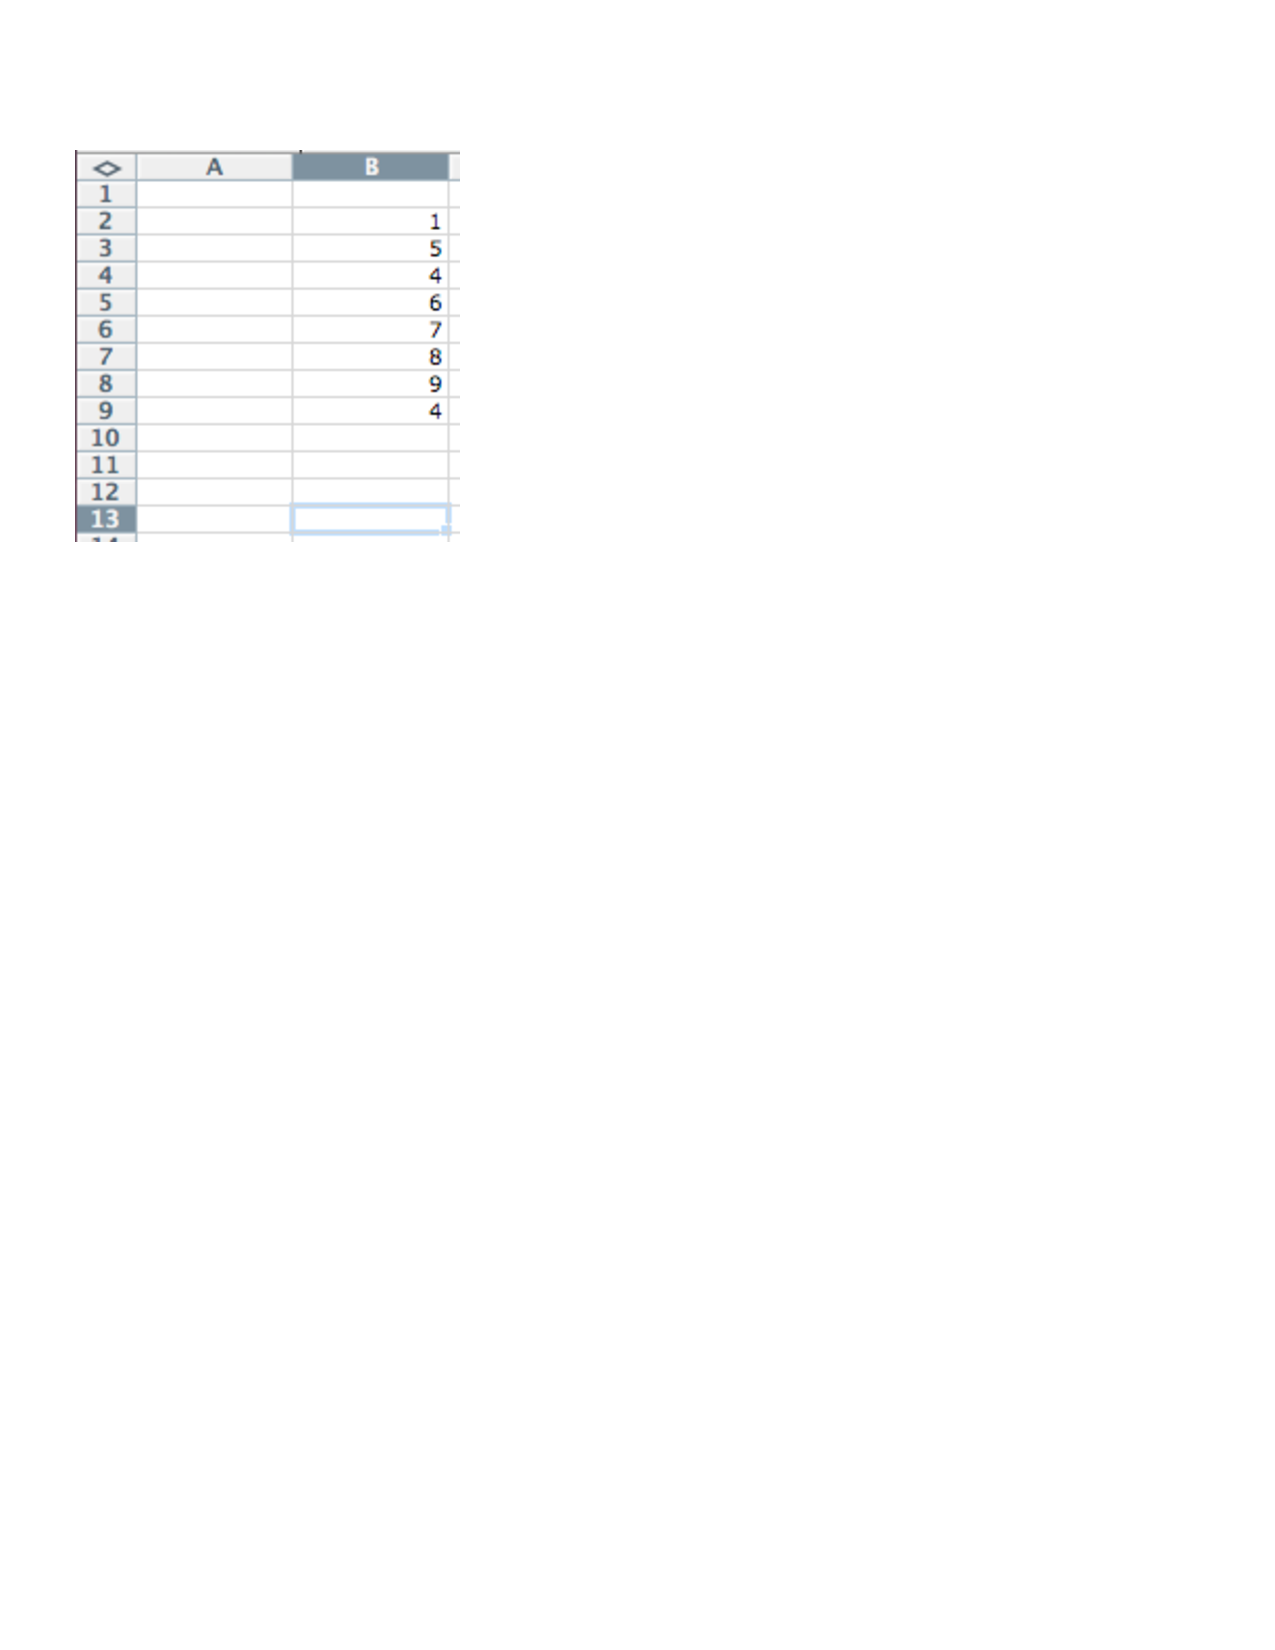
\includegraphics[width=.5\linewidth]{LabmanualFigures/Excel2.pdf}
      \caption{Inputting data}
      \label{fig:excel2}
\end{figure}

\subsection{Addressing cells}

Excel uses a Letter-Number system to address or point to specific cells. As you can see, all of the numbers in this example have been added to rows 2-9 in Column B. Using the Letter- Number system, the B2=1, B3=5, B4=4, B6=7, and so on.


\subsection{Setting one cell to equal another}

\begin{figure}
      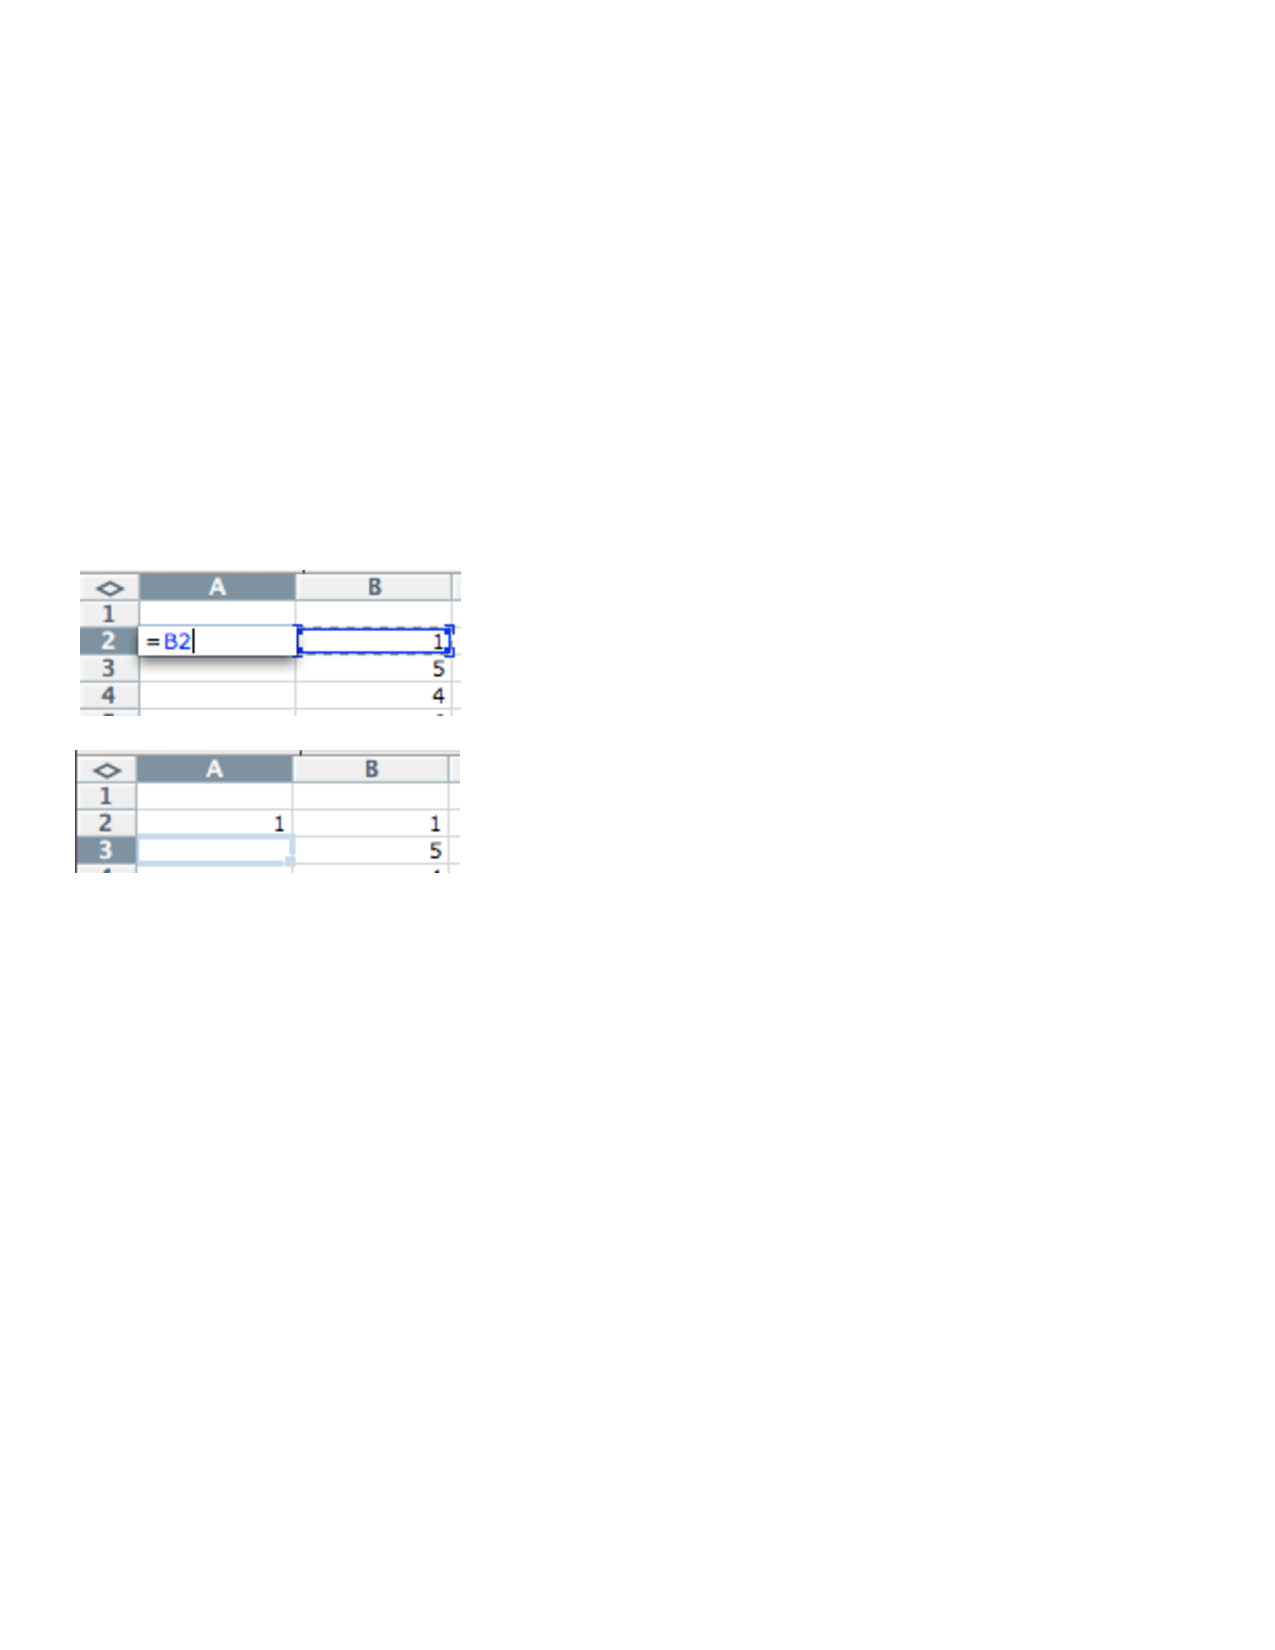
\includegraphics[width=.5\linewidth]{LabmanualFigures/Excel3.pdf}
      \caption{Making one cell equal another}
      \label{fig:excel3}
\end{figure}

If you click on an empty cell, you can make this cell have the same contents as another cell by typing the (=) sign, then clicking on the cell you want to duplicate.
E.g., click on A2, type (=), then click on B2. B2 initially had a 1 in it, now when you press enter, cell A2 will also have a 1 in it. Now if you change the contents of B2 to another number (say 5), the contents of A2 will also change to 5.
Note: this trick becomes handy later on to help you quickly manipulate data in excel

\subsection{Adding cells together, and copying commands across other cells}

\begin{figure}
      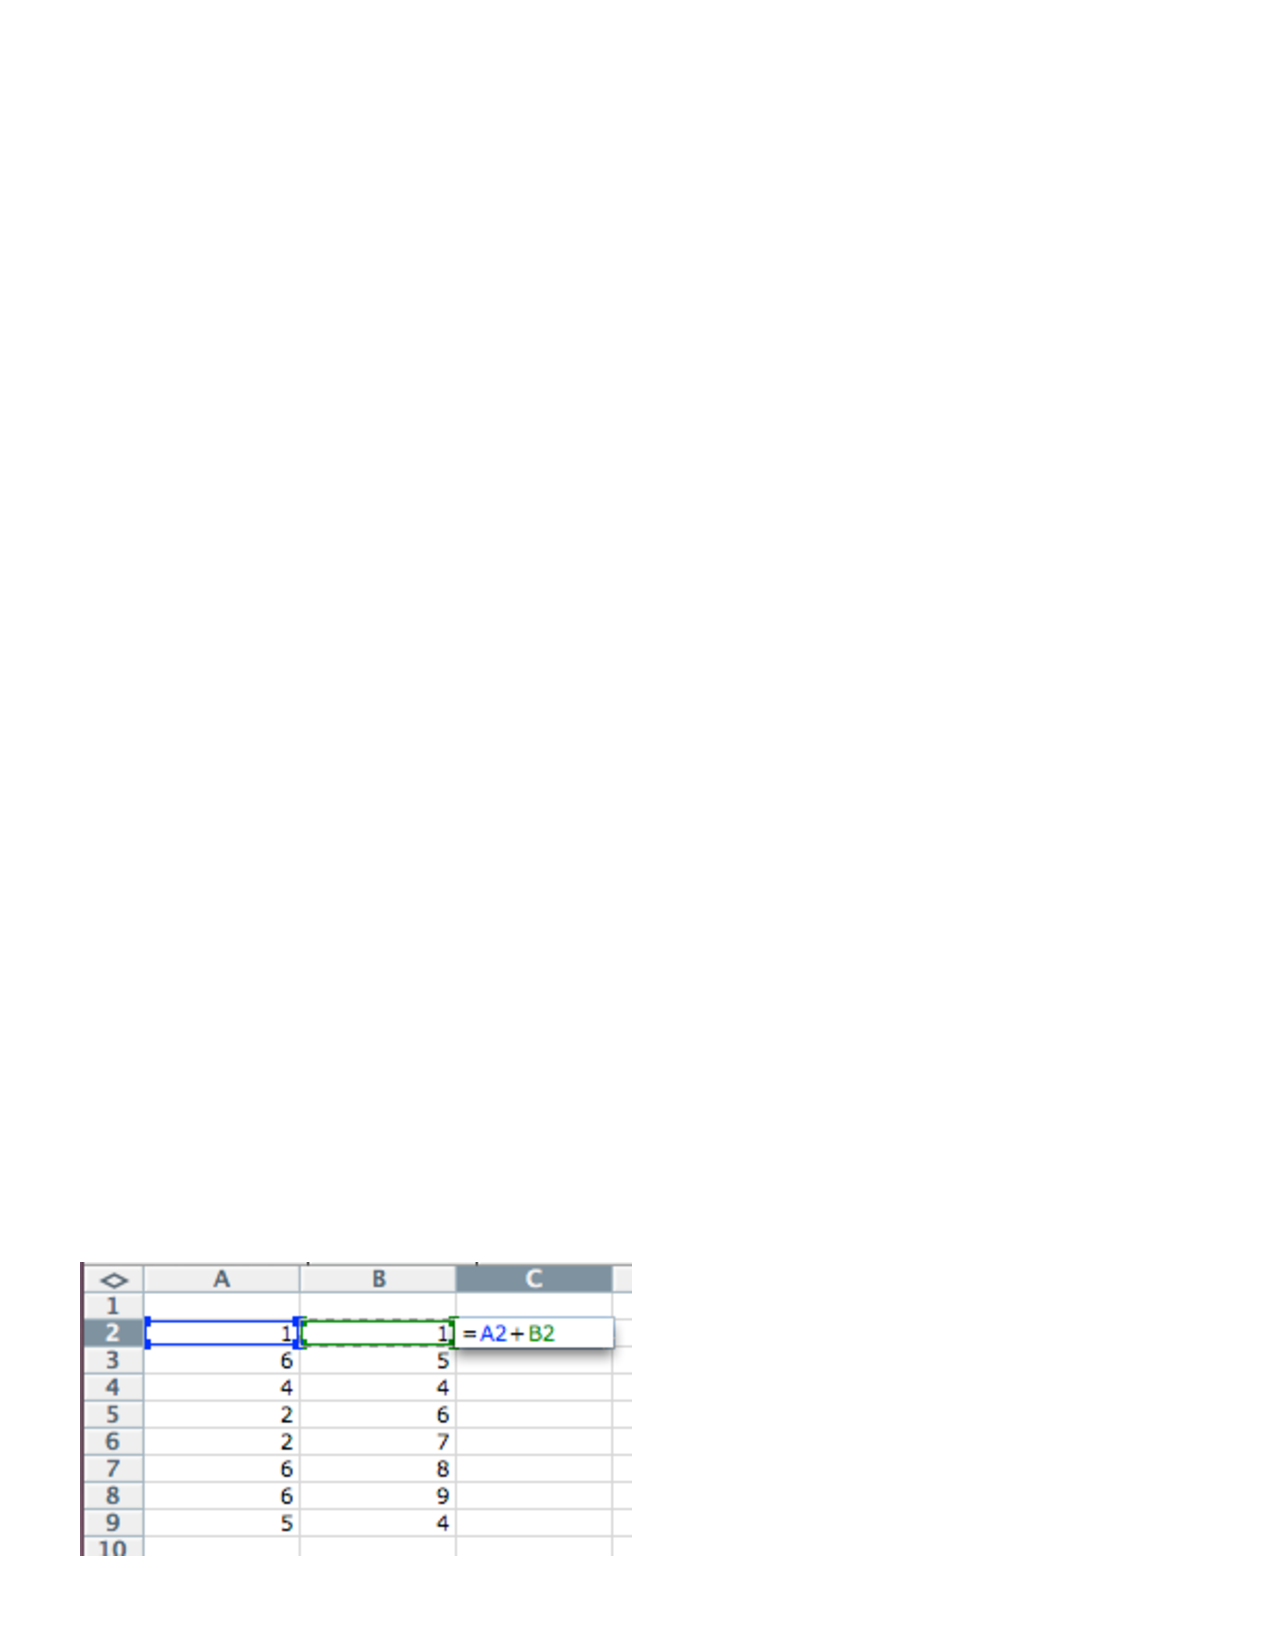
\includegraphics[width=.5\linewidth]{LabmanualFigures/Excel4.pdf}
      \caption{Adding}
      \label{fig:excel4}
\end{figure}

Let's say you had two columns of numbers. For each row you want to compute the sum of the first and second number (e.g., the first two numbers are 1 and 1, you want to add them together to get 2.
Click on a new column (C2) and type the equal sign =
Now click on A2 (which contains 1) once with the mouse, and then click on B2 (which also contains 1). Now the formula in C2 will automatically contain =A2+B2
When you press enter the two numbers will be summed, and the answer in C2 with be 2.

\begin{figure}
      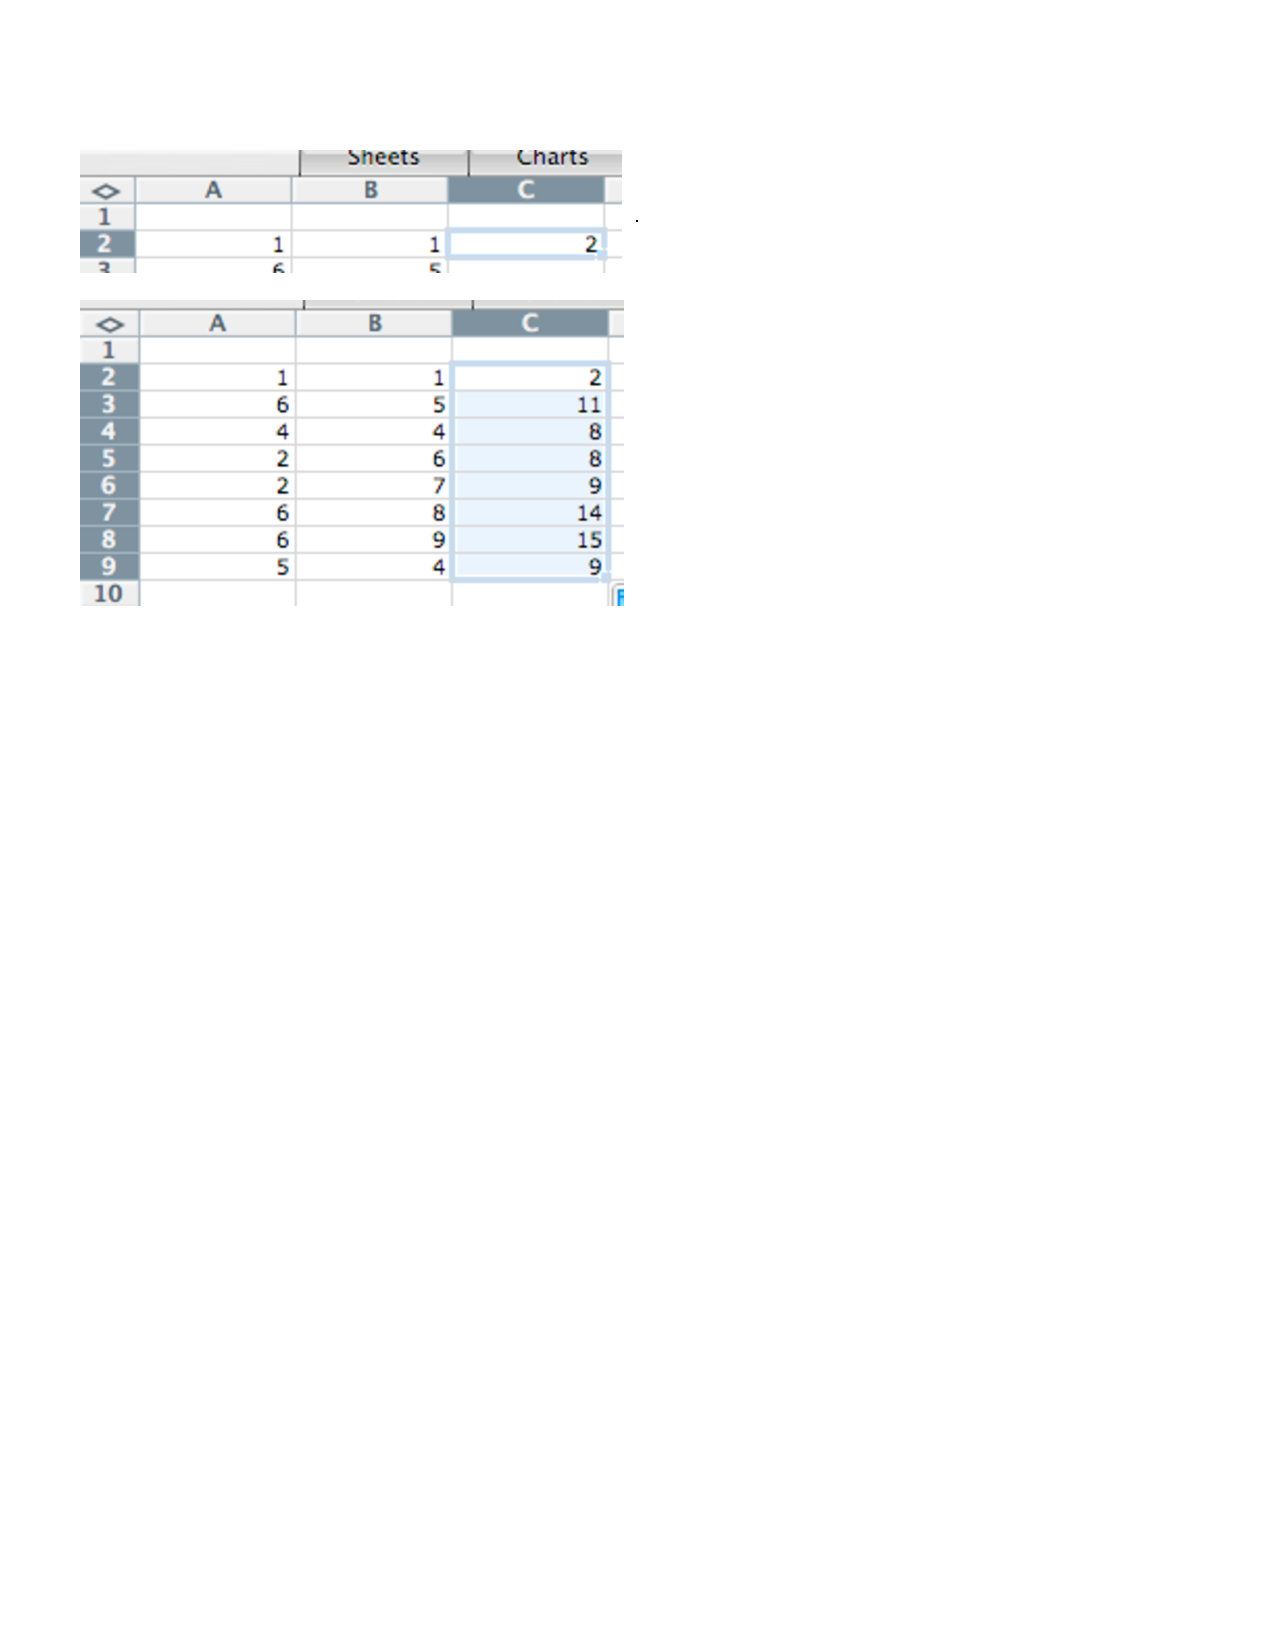
\includegraphics[width=.5\linewidth]{LabmanualFigures/Excel5.pdf}
      \caption{Applying across cells}
      \label{fig:excel5}
\end{figure}

If you want to do the same operation for all of the rows, all you have to do is click on C2. Notice there is a little blue square at the bottom right hand corner of the cell.
   

\subsection{Using a formula to add two numbers together}
You can do the same addition operation from above by using the sum formula. In this example you would click on C2, then type =sum(
Then you need to tell excel the range of columns and rows that you want to sum over. In this case you can just click on A2, and drag across to B2. This will make a temporary blue rectangle, which represents the cells that will be summed together
Complete the formula by using the )
Then press enter, and you will get the answer. 

\begin{figure}
      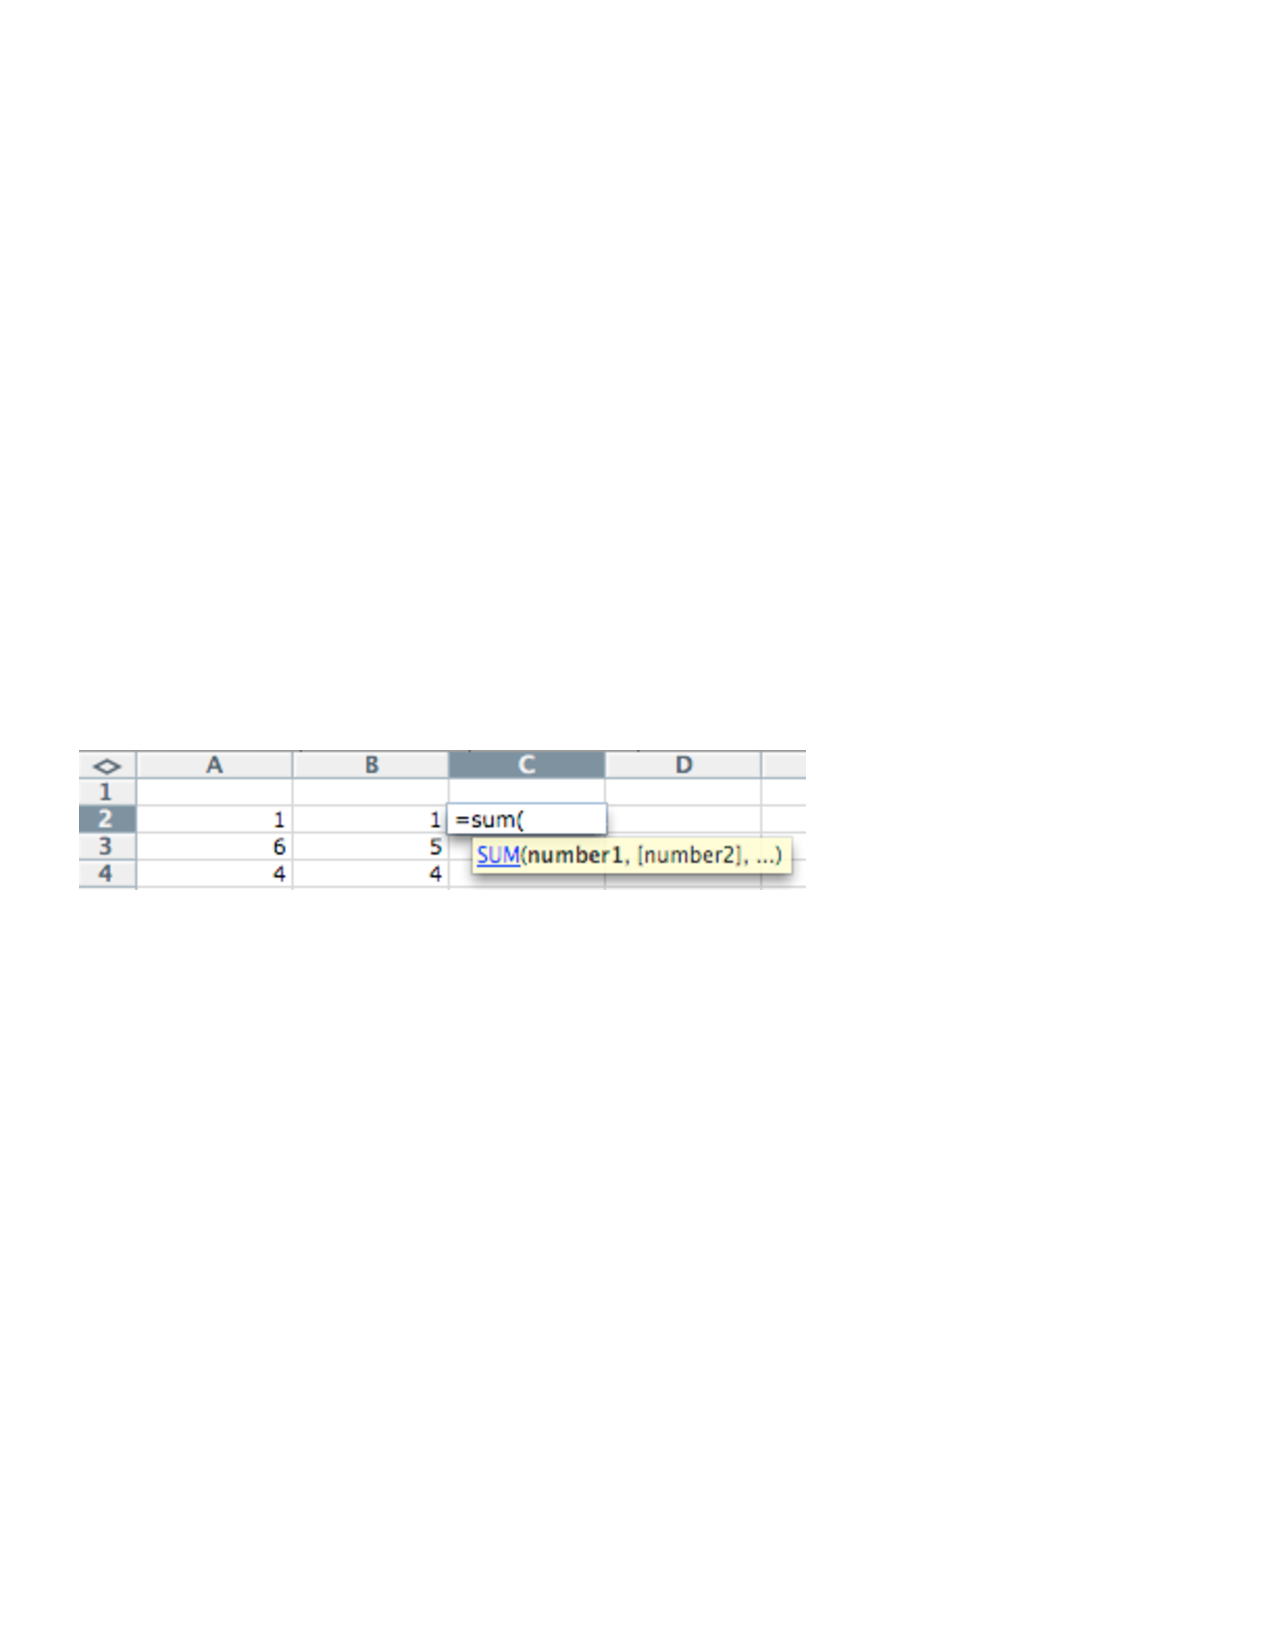
\includegraphics[width=.5\linewidth]{LabmanualFigures/Excel6.pdf}
      \caption{Adding using the sum formula}
      \label{fig:excel6}
\end{figure}

You can also copy this formula down across the other cells in the same way as above
If you click on the little square, then drag down, the formula will be applied to each of the rows.
And, then you have all the answers without having to enter the formula separately for each row.

\begin{figure}
      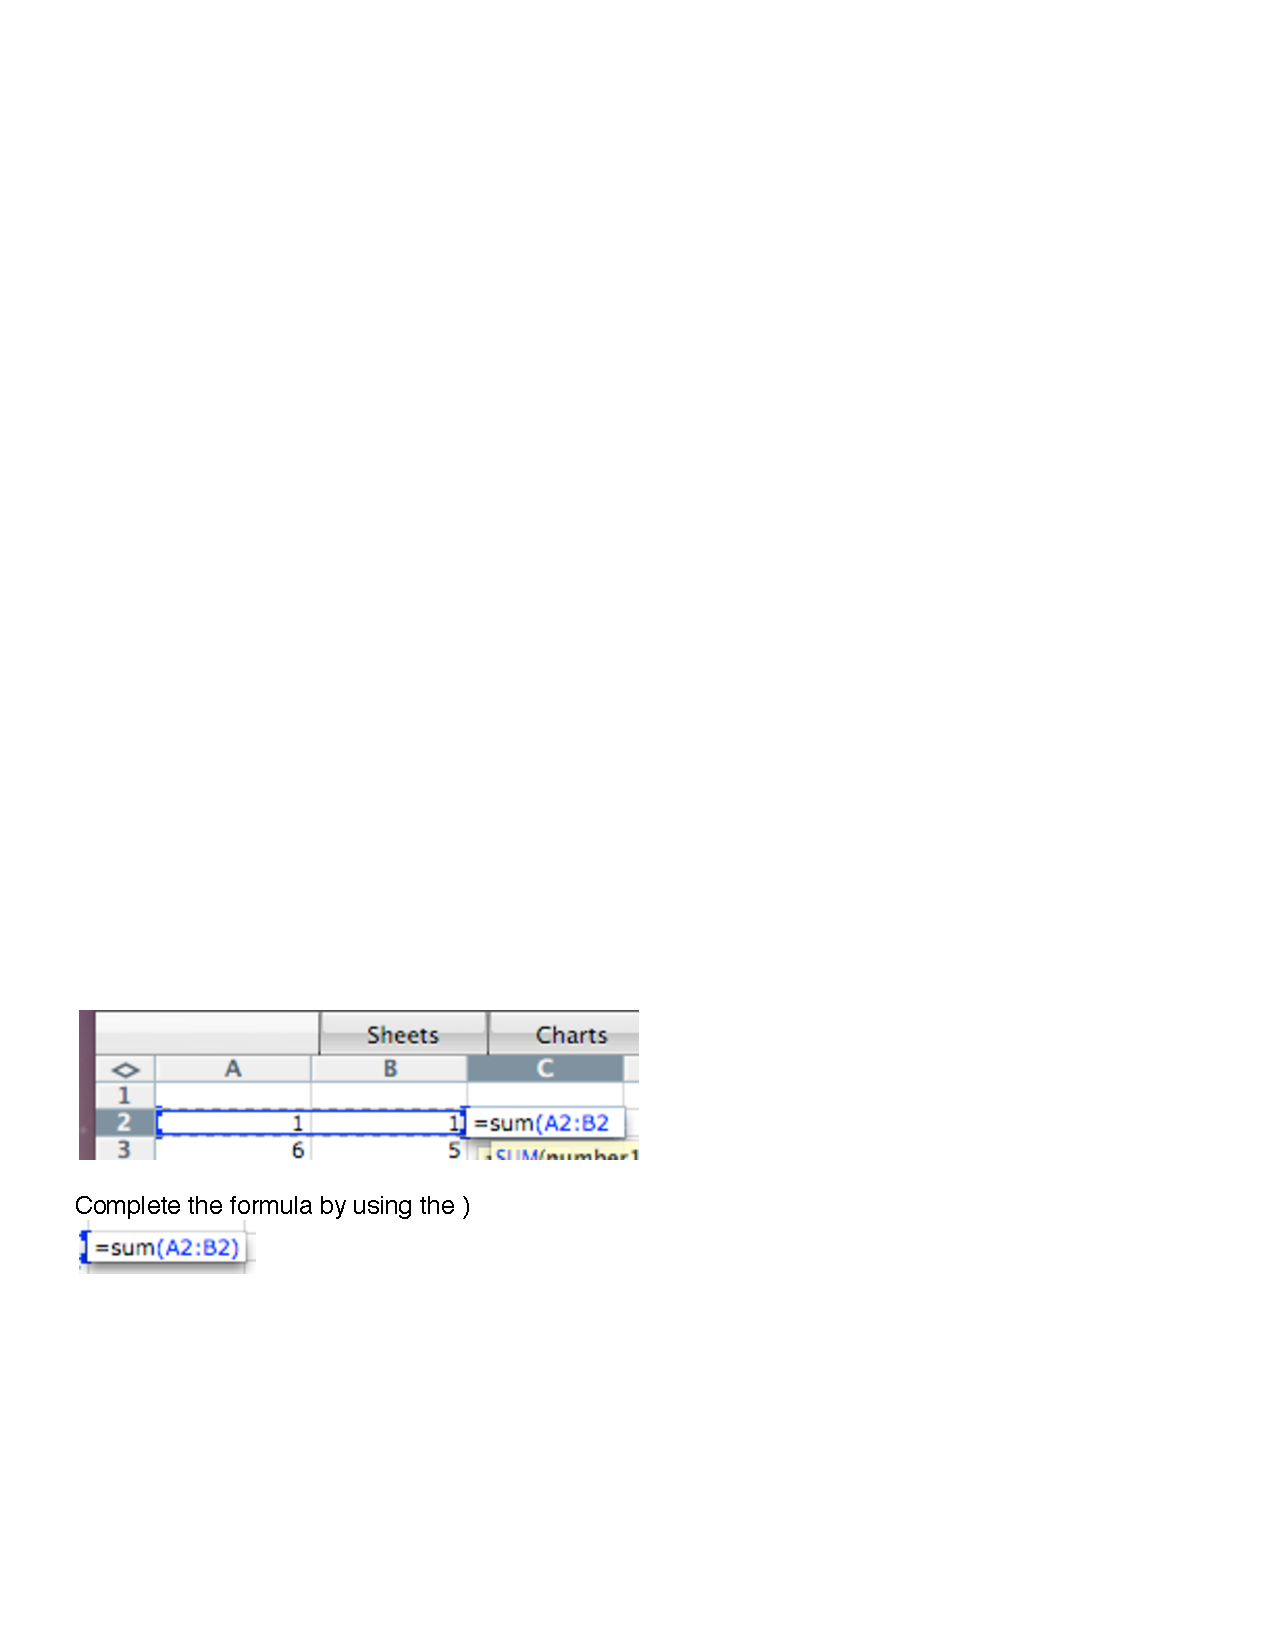
\includegraphics[width=.5\linewidth]{LabmanualFigures/Excel7.pdf}
      \caption{Completing the formula}
      \label{fig:excel7}
\end{figure}    

\subsection{Getting an average}

Using the same method as the sum formula, you can also compute the mean of a set of numbers by using the average function instead of the sum function. The process is the same. Select a cell, type =average( then select the cells you want (in the example B2:B9) and press enter.

\begin{figure}
      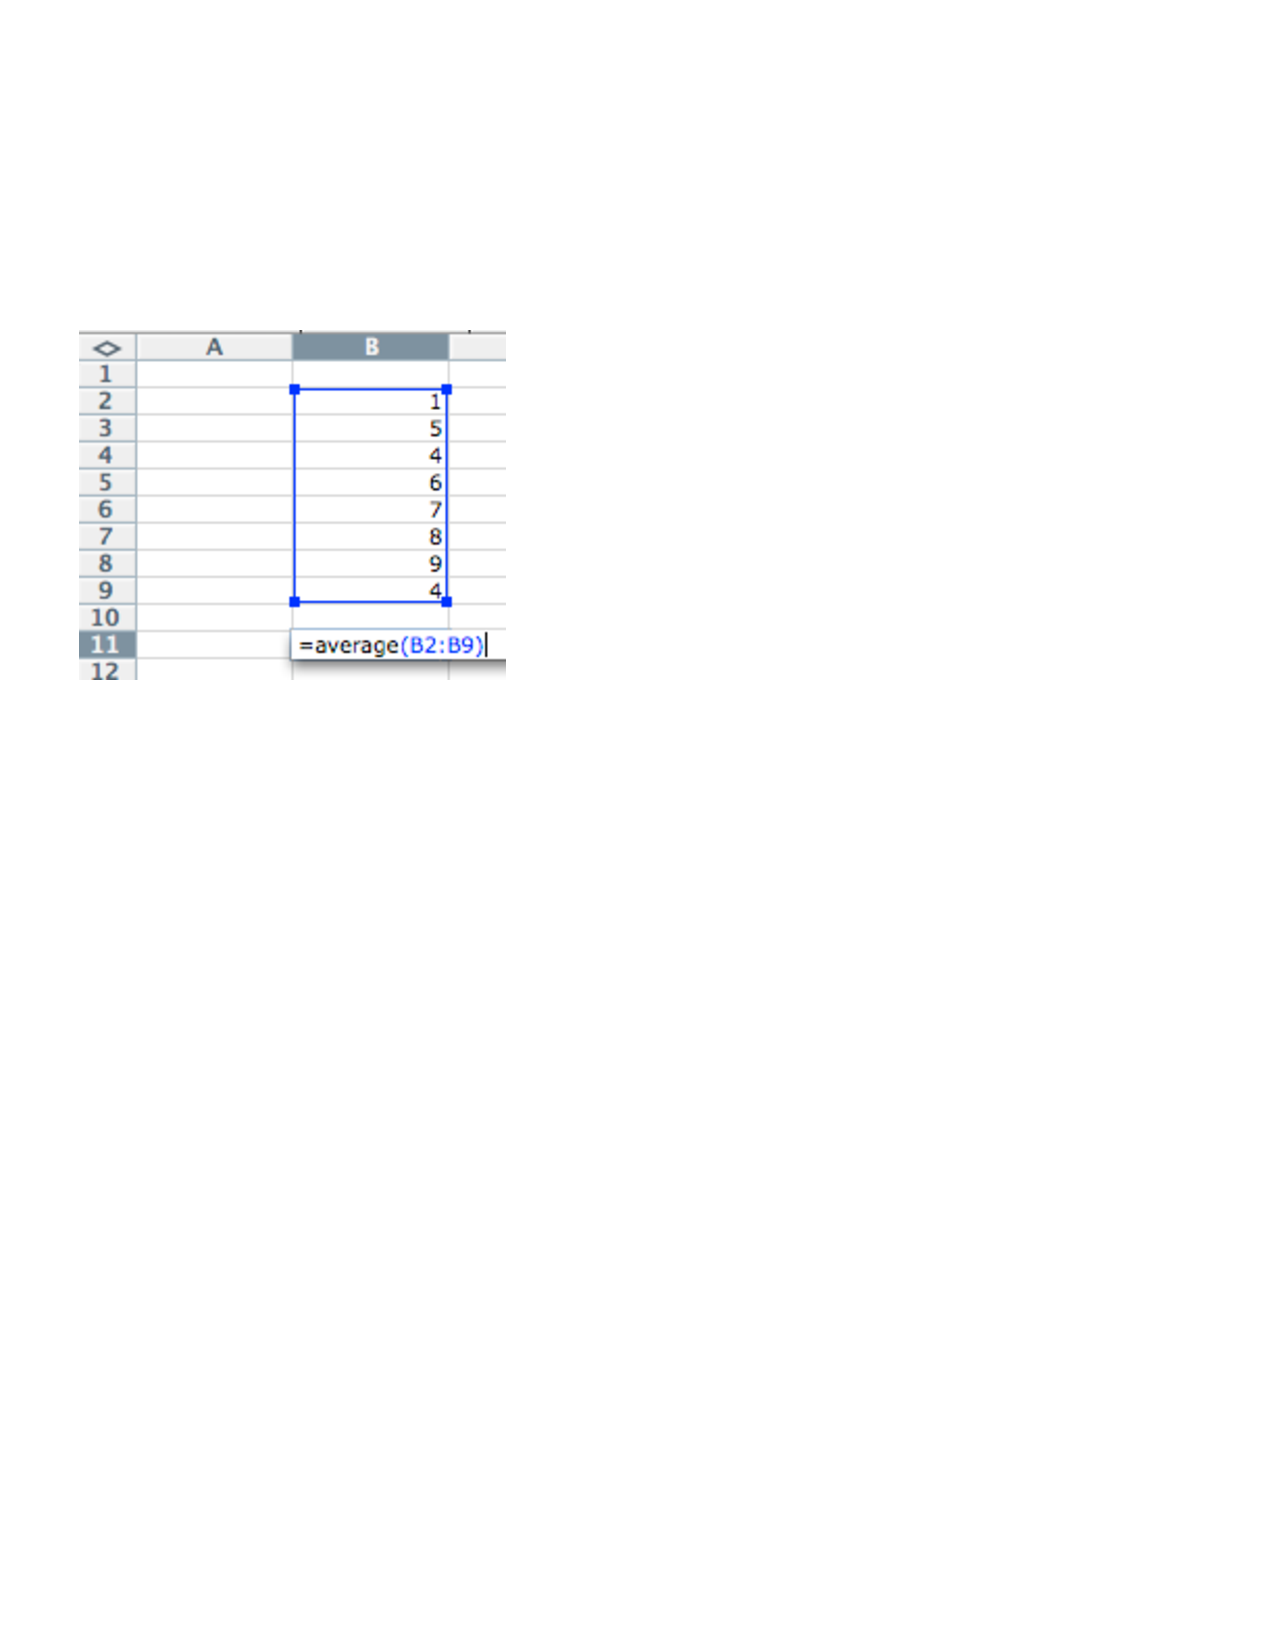
\includegraphics[width=.5\linewidth]{LabmanualFigures/Excel8.pdf}
      \caption{The average formal}
      \label{fig:excel8}
\end{figure}

\subsection{Other formulas}

\begin{itemize}
\item Max – finds the biggest number
\item Min- finds the smallest number
\item Stdev- computes the standard deviation
\item Countif – counts the number of times a specific value occurs
\end{itemize}

Excel has a dictionary of other functions that may be useful, you can look them using help, or using insert: function, from the menu.


\subsection{Selecting a range of cells}
Formulas usually require you to enter a range of cells to compute. The format is put the upperleftmost cell first (e.g., A2), and then the bottomrightmost cell last (e.g., C9). So, A2:C9 would signify the
following rectangle.

\begin{figure}
      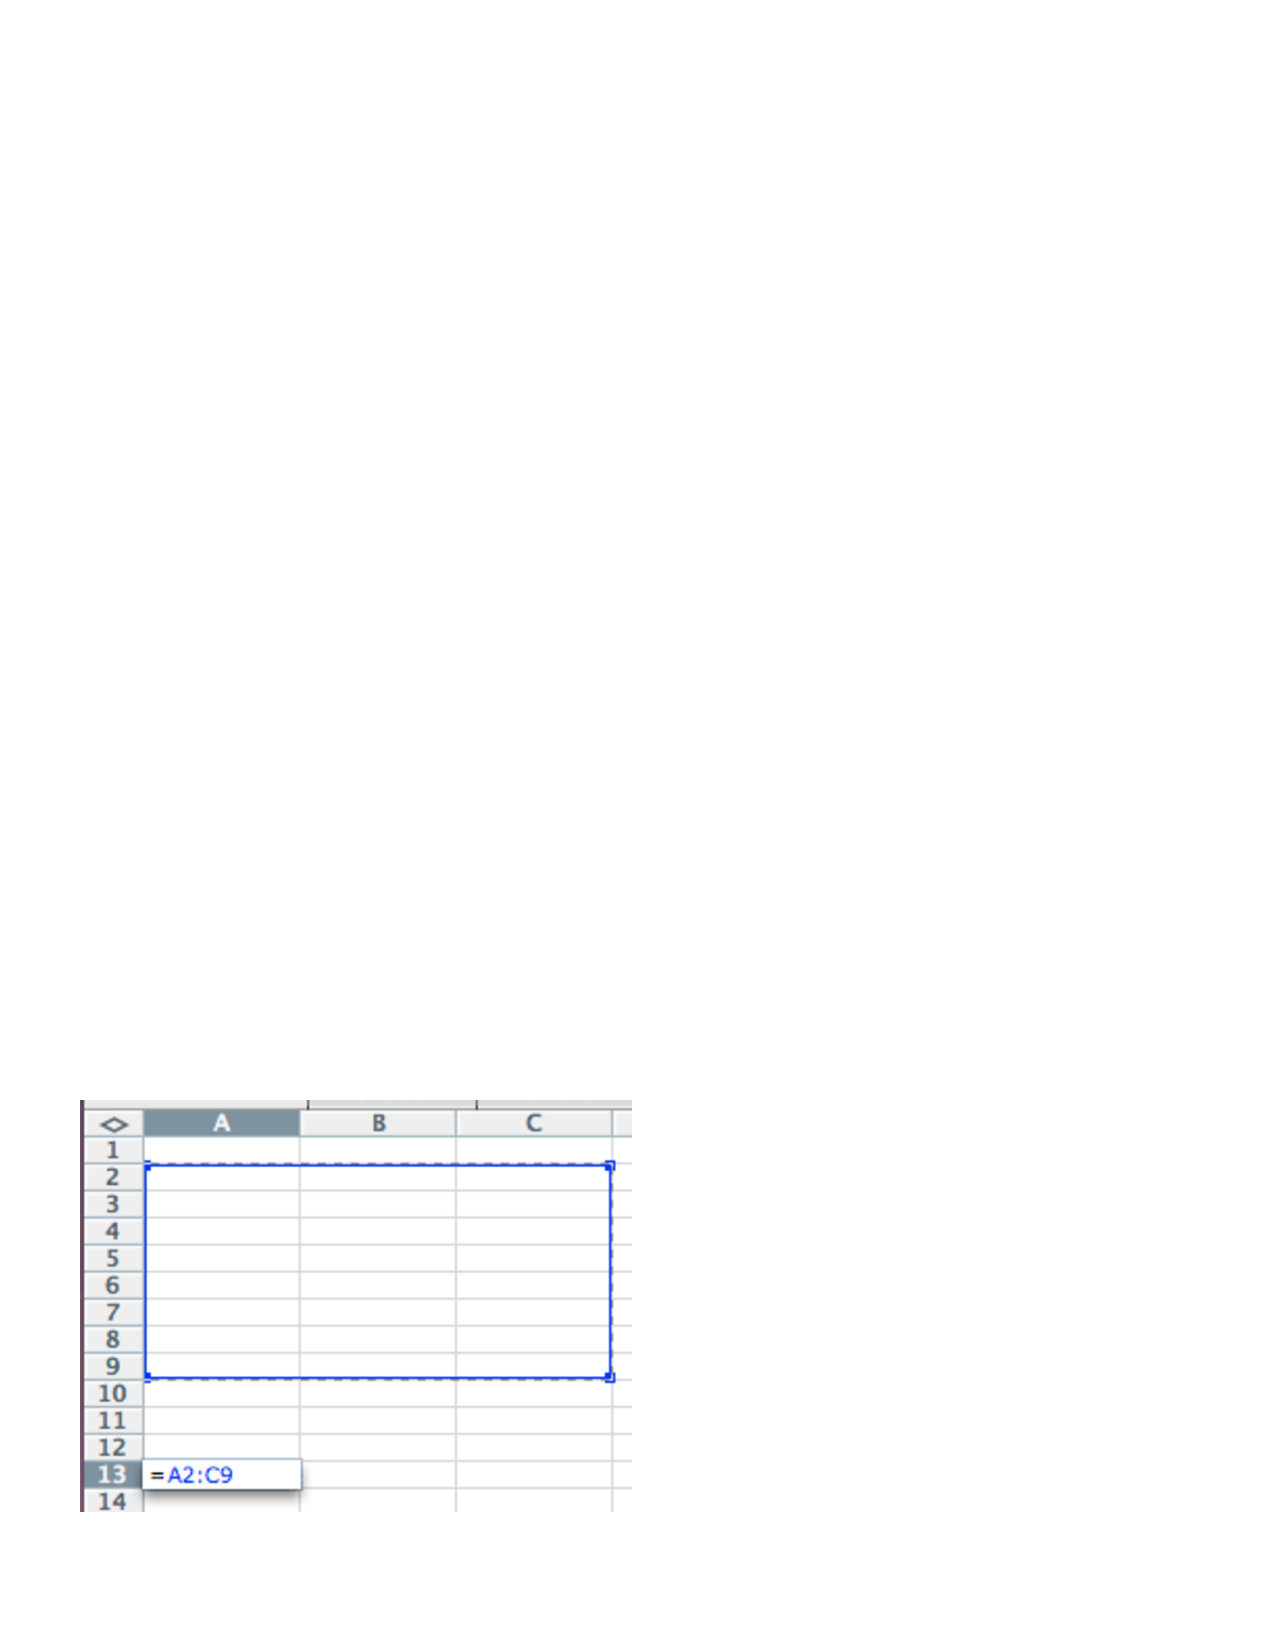
\includegraphics[width=.5\linewidth]{LabmanualFigures/Excel9.pdf}
      \caption{selecting a range}
      \label{fig:excel9}
\end{figure}
  

\subsection{Copying a formula to another cell: relative coordinates}

If you were to now select cell A13 it would have the formula =A2:C9 inside. If you copied this cell, and then pasted it into the cell beside it A14, Excel would automatically move the rectangle over one. This is because without further specification, excel always treats cells in relative coordinates.

\begin{figure}
      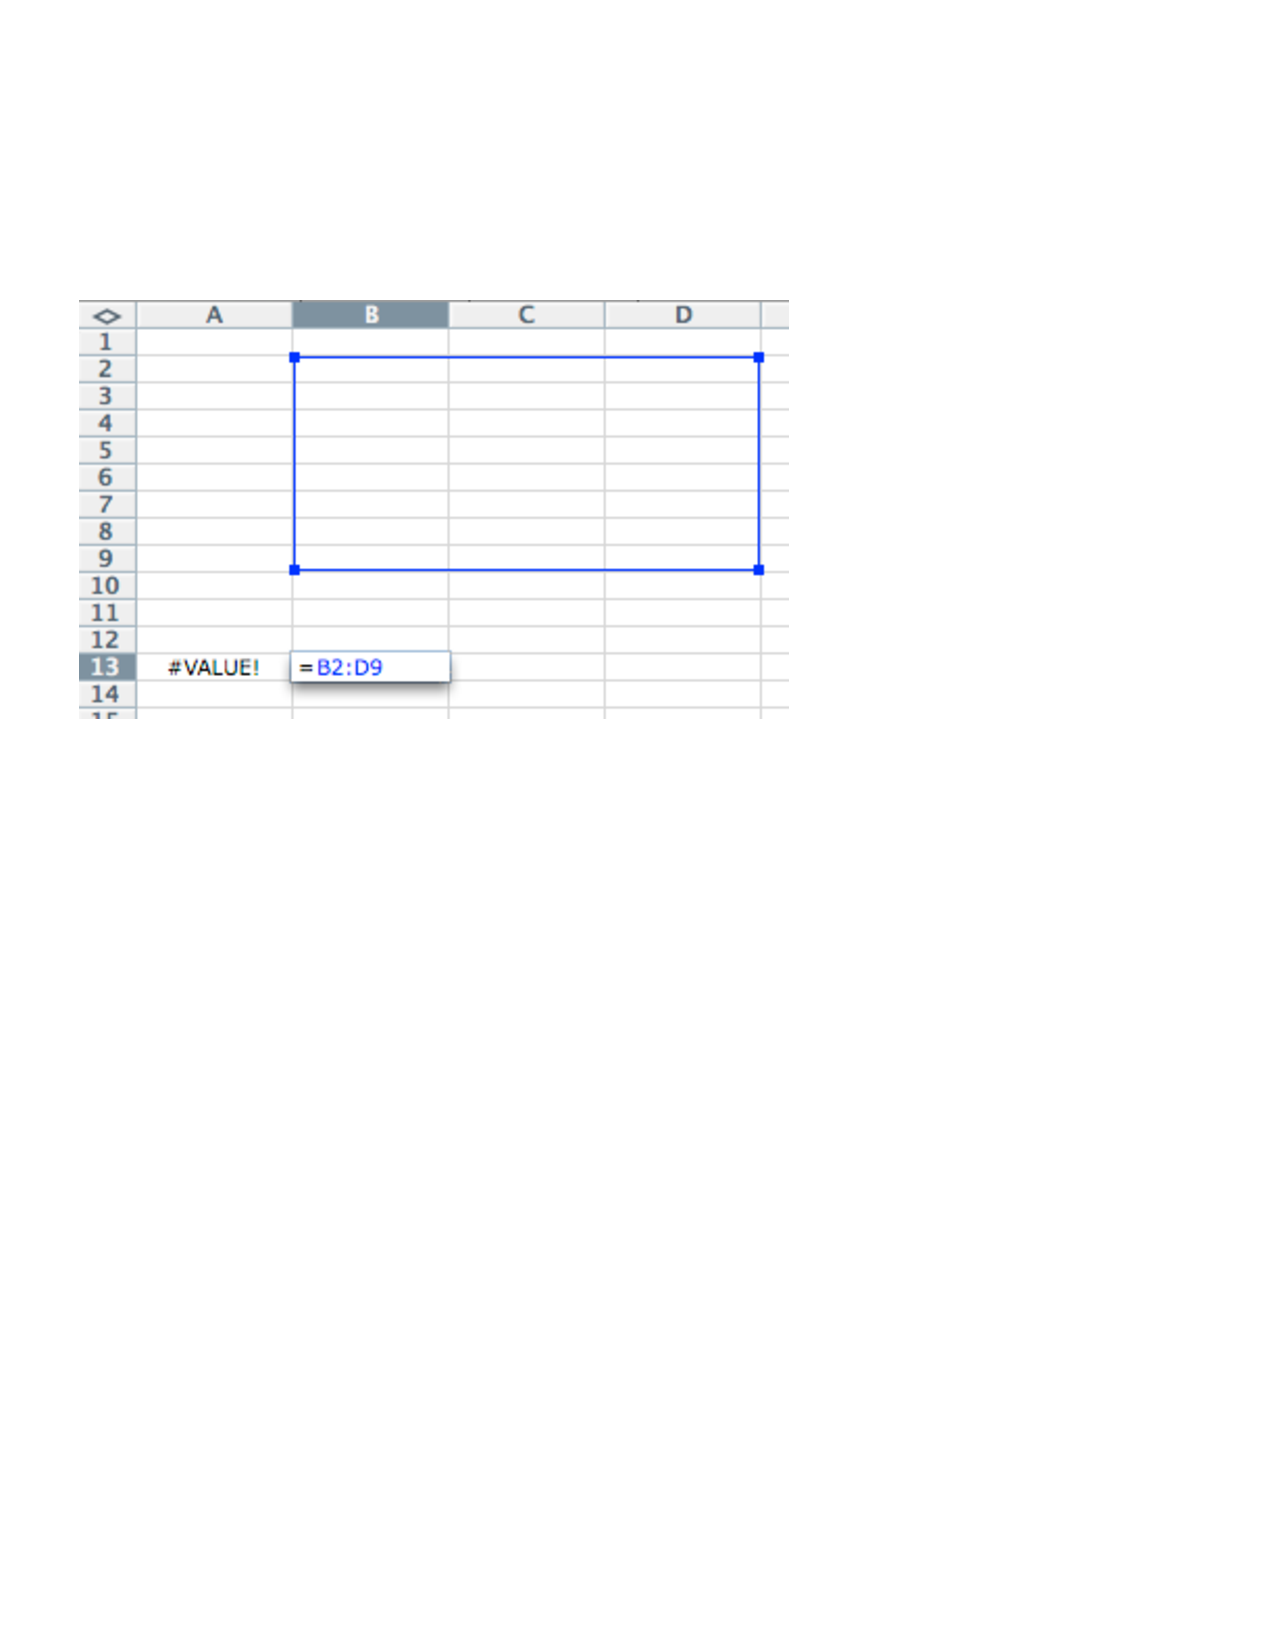
\includegraphics[width=.5\linewidth]{LabmanualFigures/Excel10.pdf}
      \caption{Relative coordinates}
      \label{fig:excel10}
\end{figure}
 

\subsection{Absolute coordinates}
You can control whether or not excel uses relative coordinates. When you set the range you can insert the \$ sign to make sure that excel holds the rectangle in place.
For example:
A13 =A2:C9
-this formula has no \$s, as in the above example, if you copy this formula to another cell say
B13, then B13=B2:D9, and not the original A2:C9
A13=\$A\$2:\$C\$9
-This formula has \$s infront of both letter and number for each cell in the rectangle. Now, when
the formula is copied to another cell, the original rectangle will be used. E.g., B13=A2:C9 You can set the only columns or the row or both to absolute coordinates using the \$ sign.
 

\subsection{Sorting data}

\begin{figure}
      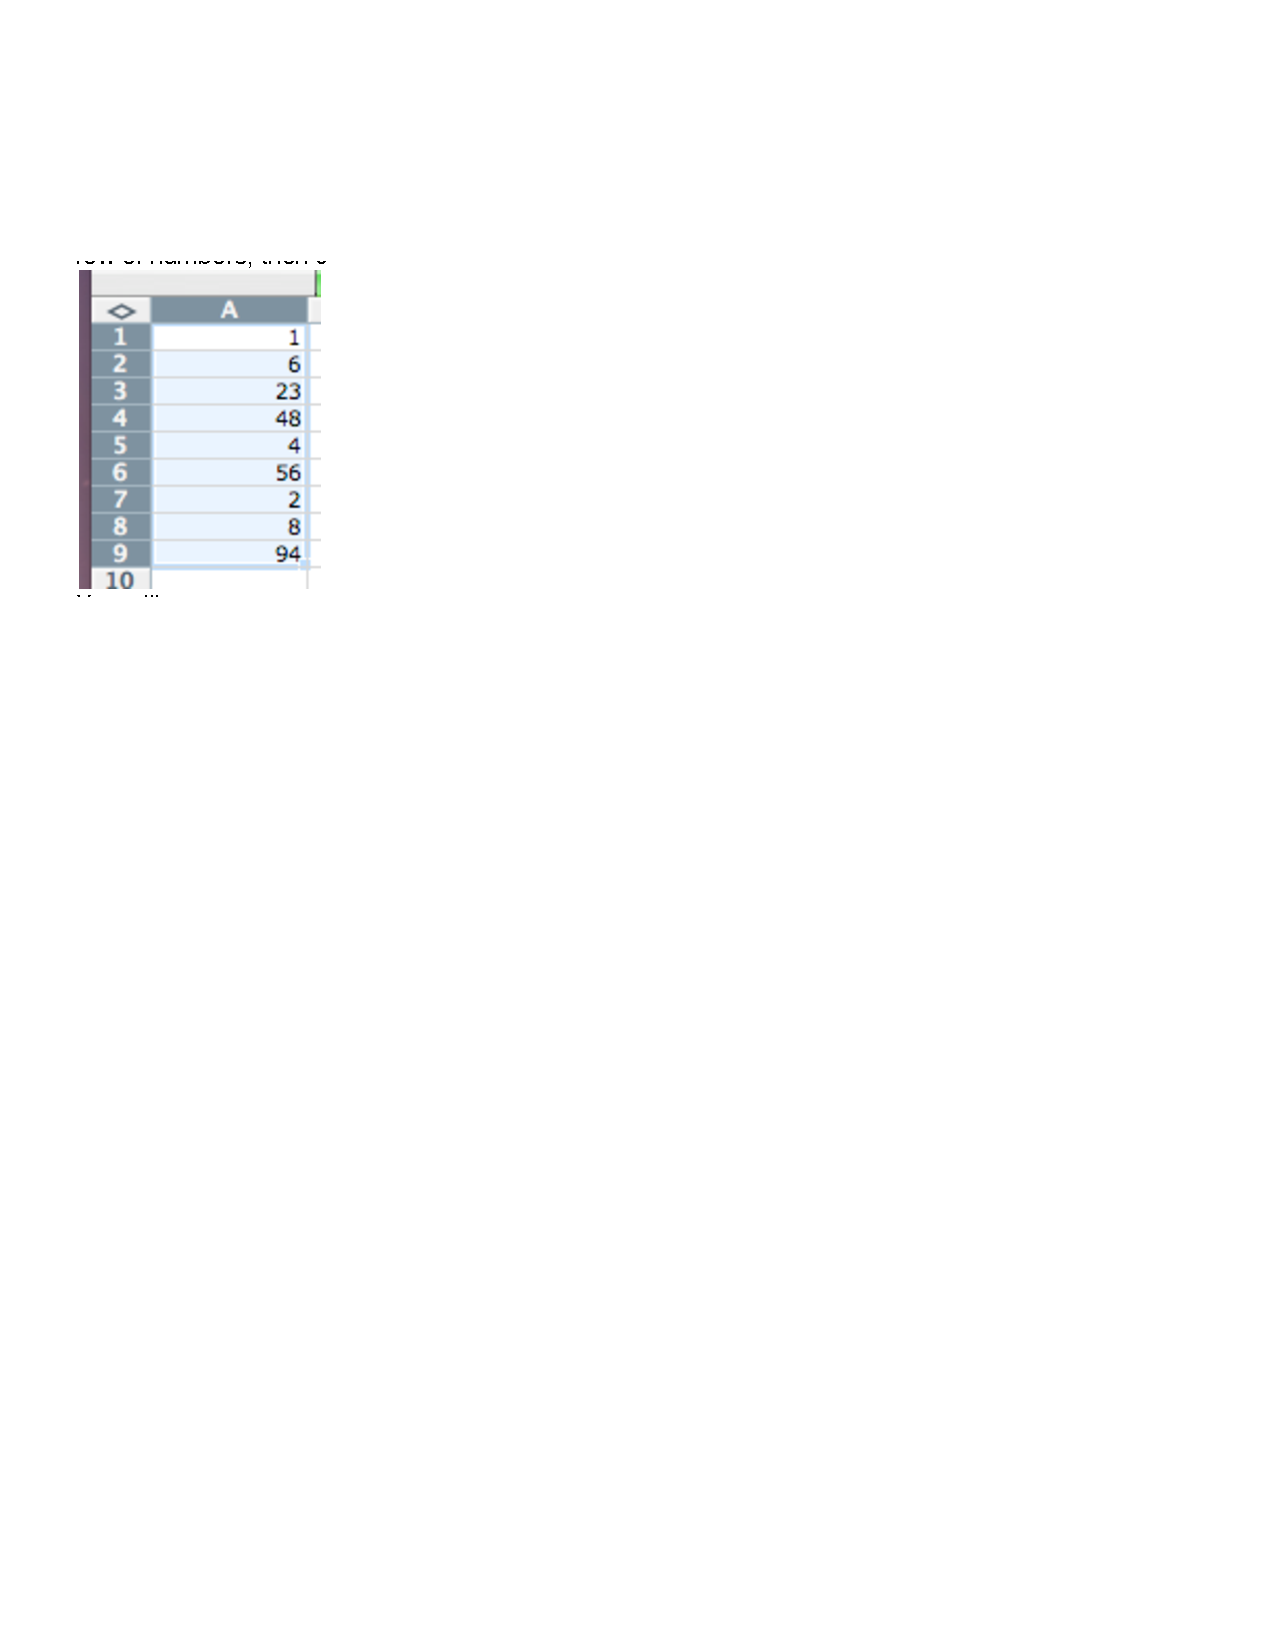
\includegraphics[width=.5\linewidth]{LabmanualFigures/Excel11.pdf}
      \caption{Some numbers to sort}
      \label{fig:excel11}
\end{figure}
 

If you had a bunch of numbers in random order, you could easily sort them by selecting the column or row of numbers, then click on Data from the menu, and choose sort:

\begin{figure}
      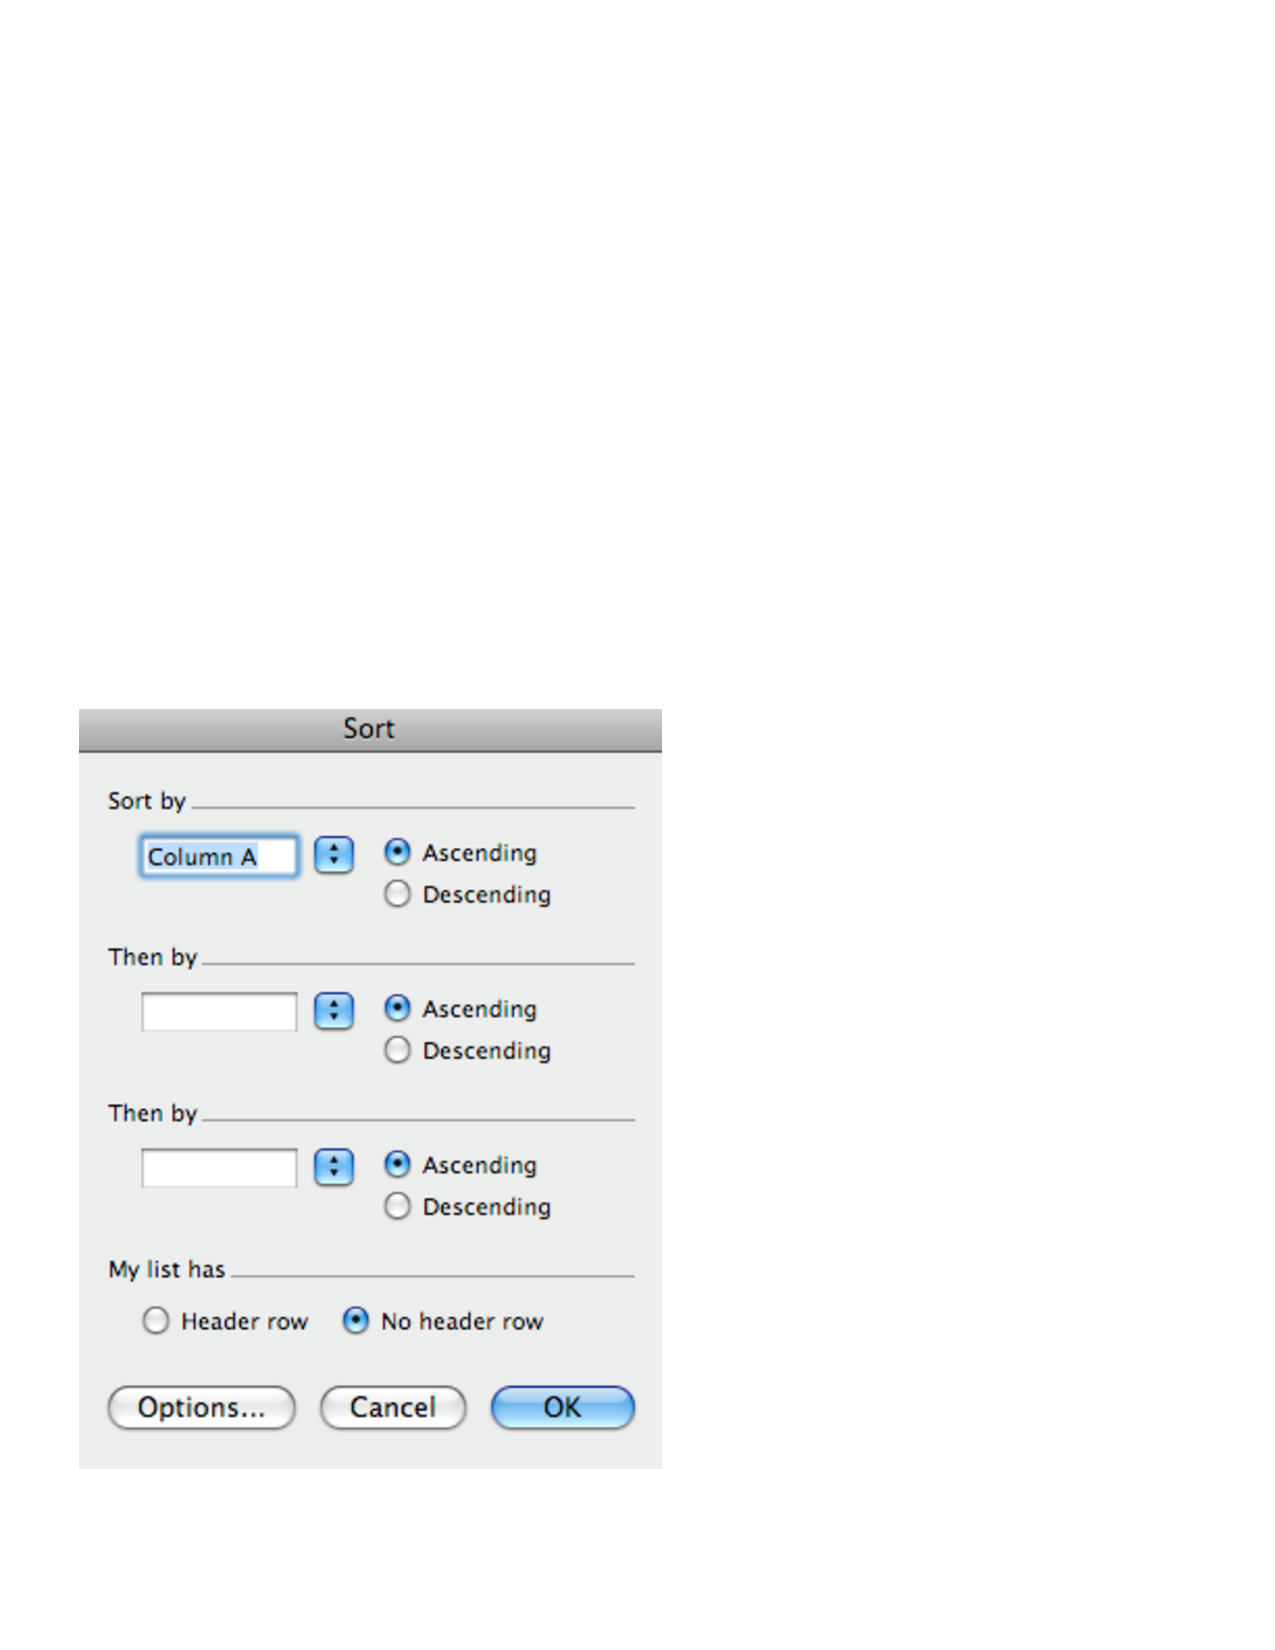
\includegraphics[width=.5\linewidth]{LabmanualFigures/Excel12.pdf}
      \caption{Sorting}
      \label{fig:excel12}
\end{figure}
 


 
You will see a menu something like this. You can choose to sort the current column ascending (smallest to largest) or descending (largest to smallest). Click OK and the data will be rearranged in order.
  

\subsection{Making a histogram}

\begin{figure}
      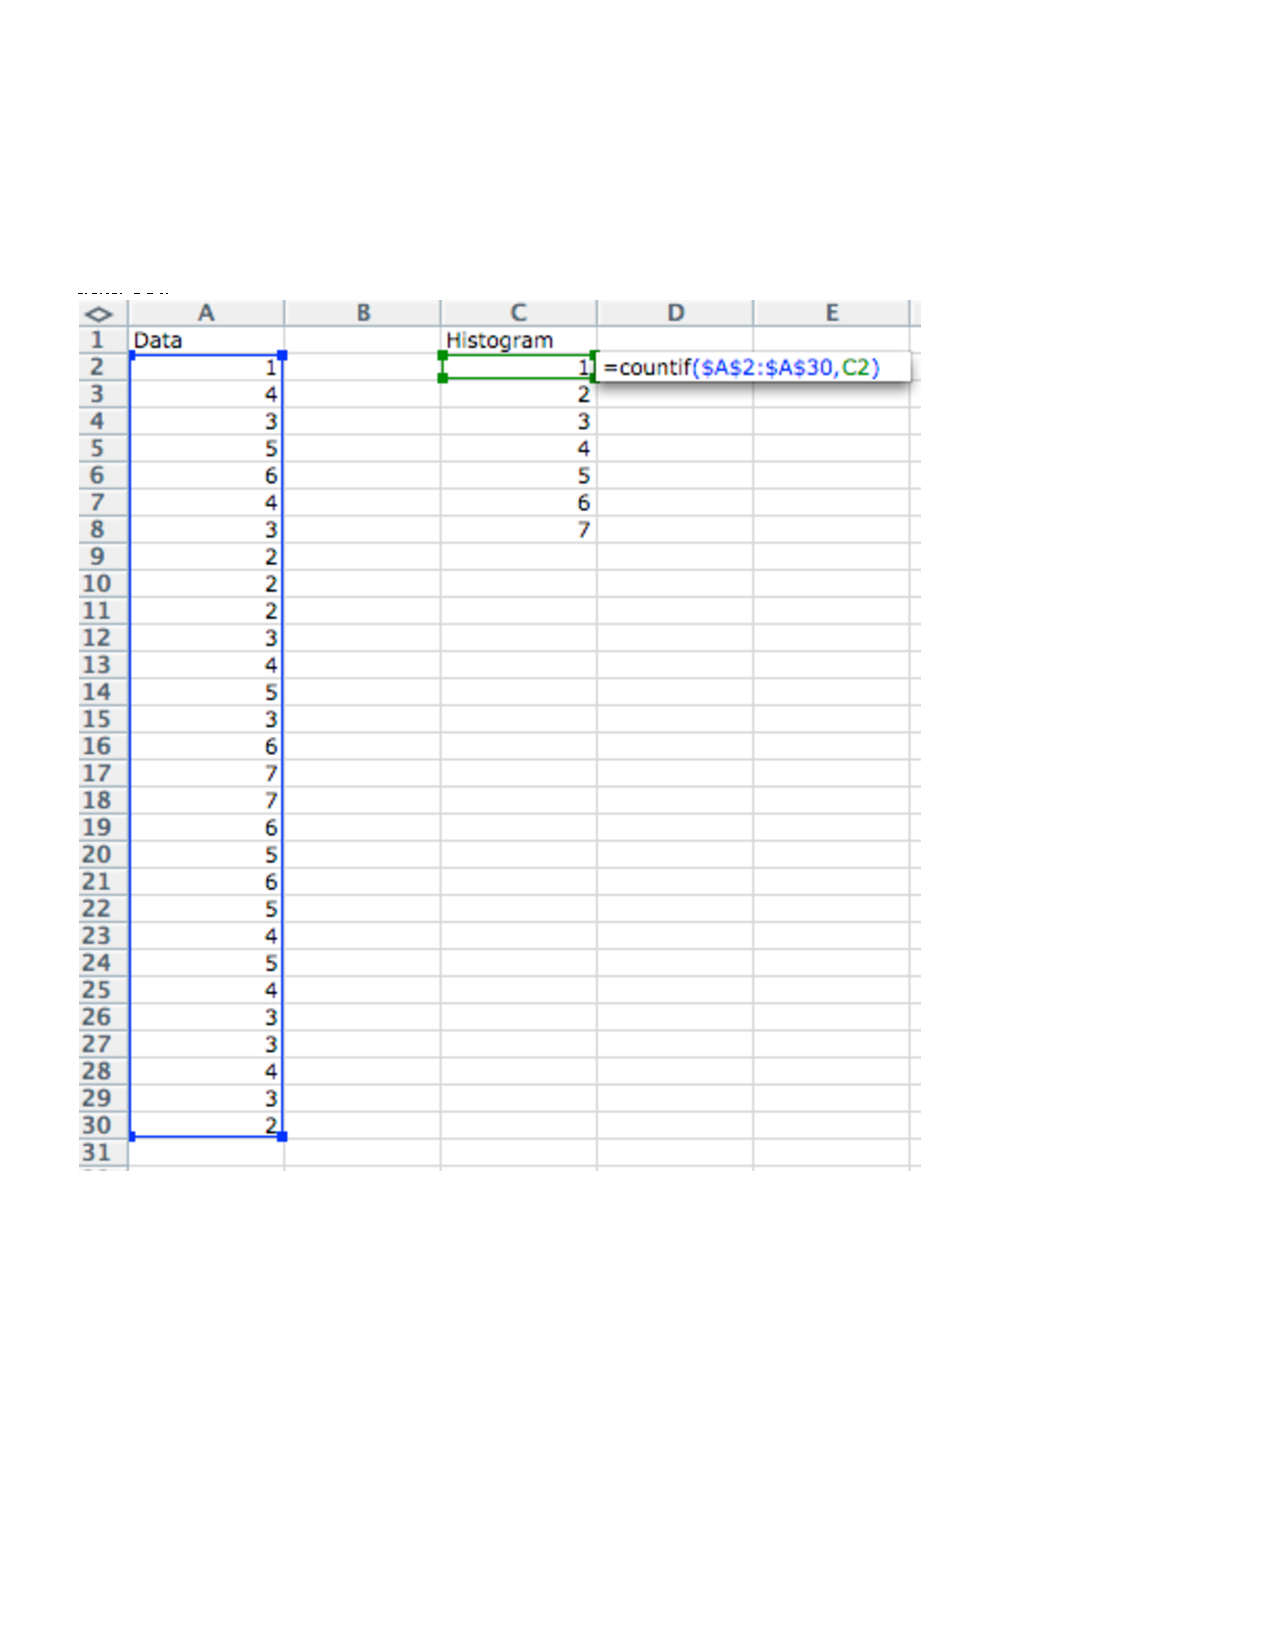
\includegraphics[width=.7\linewidth]{LabmanualFigures/Excel13.pdf}
      \caption{Making a histogram}
      \label{fig:excel13}
\end{figure}
 


If you want to know how many responses occurred for a particular range of values you can create a histogram. The following example is a very simple way to count individual categories of values in a data set.
Column A has the example data. In column C, I created cells with values ranging from 1 to 7 (Cells C2 : C8). In cell D2, I typed in the countif(range,value) formula. The range refers to the selected data (\$A\$2:\$A\$30). 

Note, there are \$ signs used before the letter and numbers so that the selected data will be the same when the formula is copied. In this case, it is the value 1, which is in Cell C2. The value refers to the entity that is being counted. When you press enter, excel will compute the number of times that 1 appears in the data. You can now drag cell (D2) with the formula down, and it will be used to count the rest of the numbers.
 


\subsection{Making a table}

\begin{figure}
      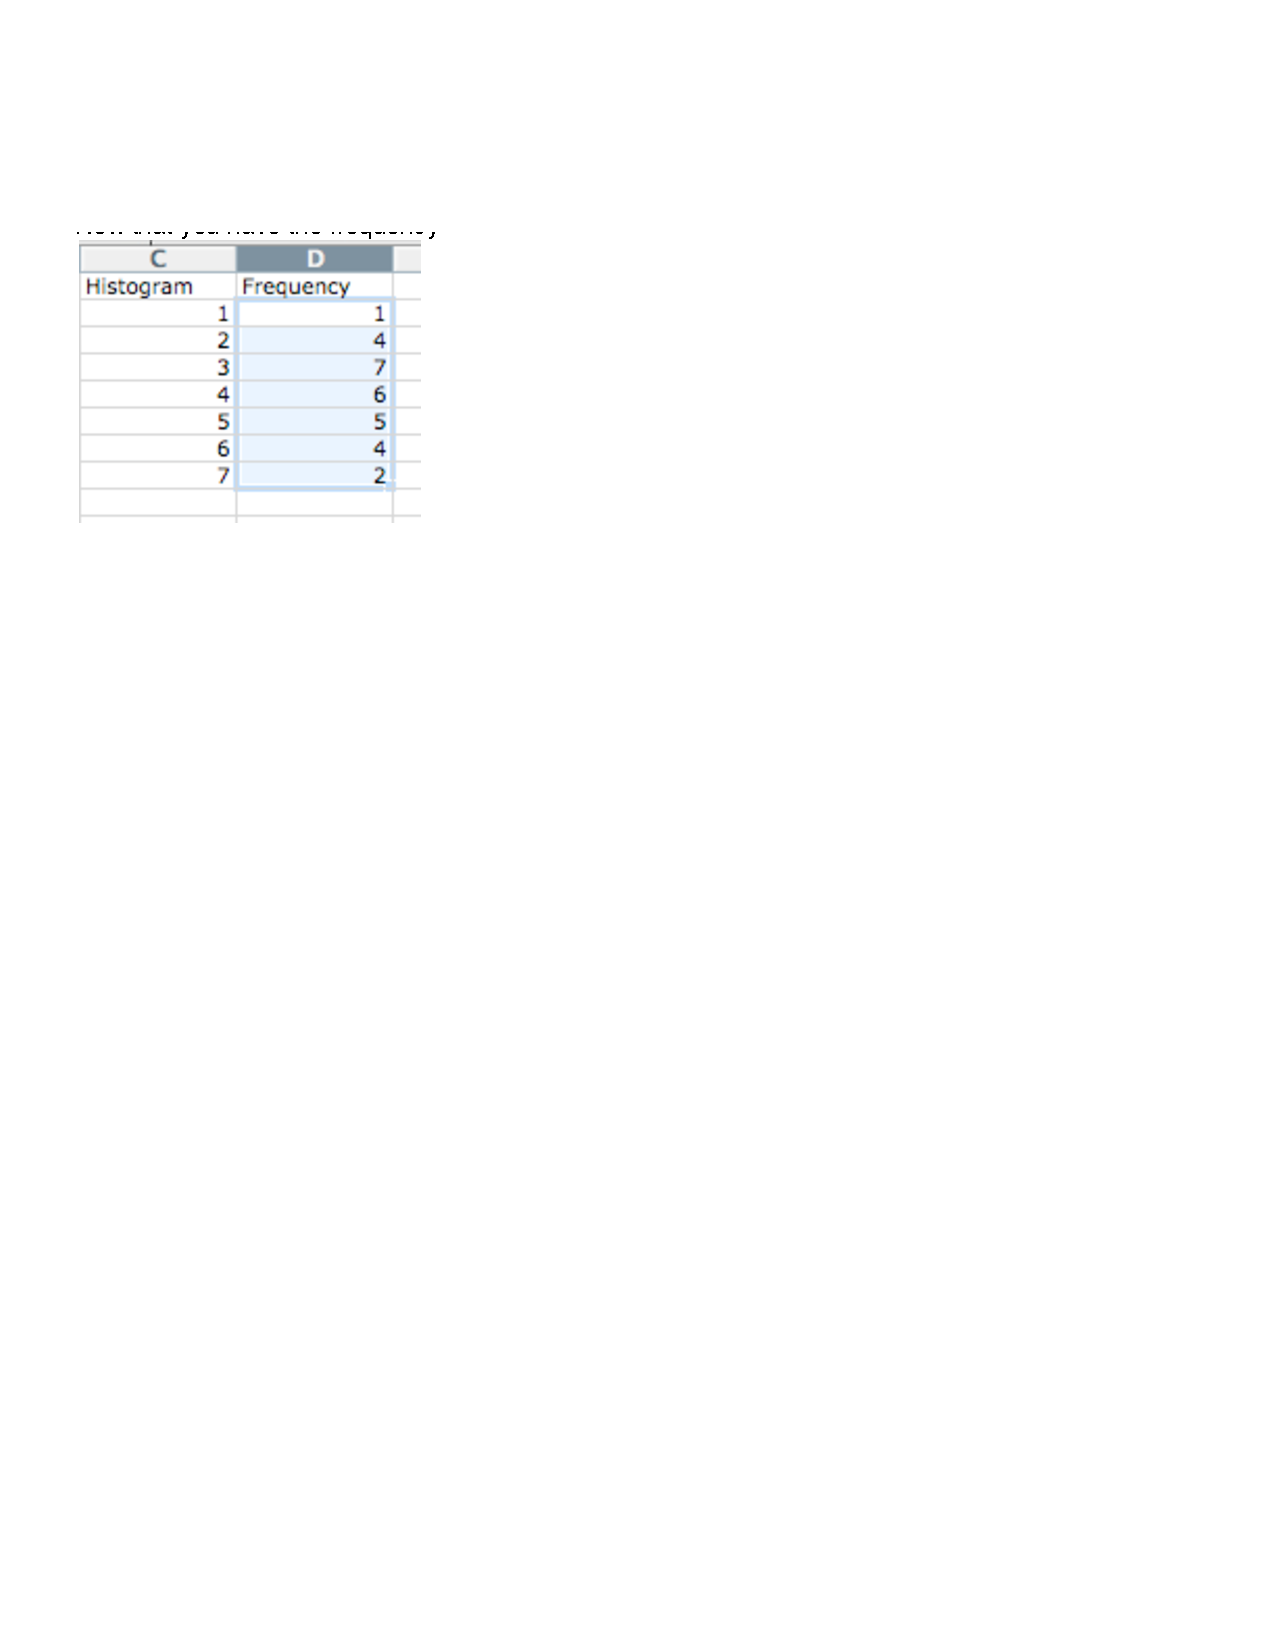
\includegraphics[width=.7\linewidth]{LabmanualFigures/Excel14.pdf}
      \caption{Making a table}
      \label{fig:excel14}
\end{figure}
 
Now that you have the frequency of each of the values from 1-7.
You can make a graph by selecting the column with the frequencies in it, and then click on INSERT, from the menu, and choose chart. Select a column chart, and then you will see:
You can then edit this chart. You should insert a title for the figure, an x-axis label (e.g., the numbers on the bottom represent different categories from the data), and a y-axis label (the numbers on the left side represent the frequency count).
 

\begin{figure}
      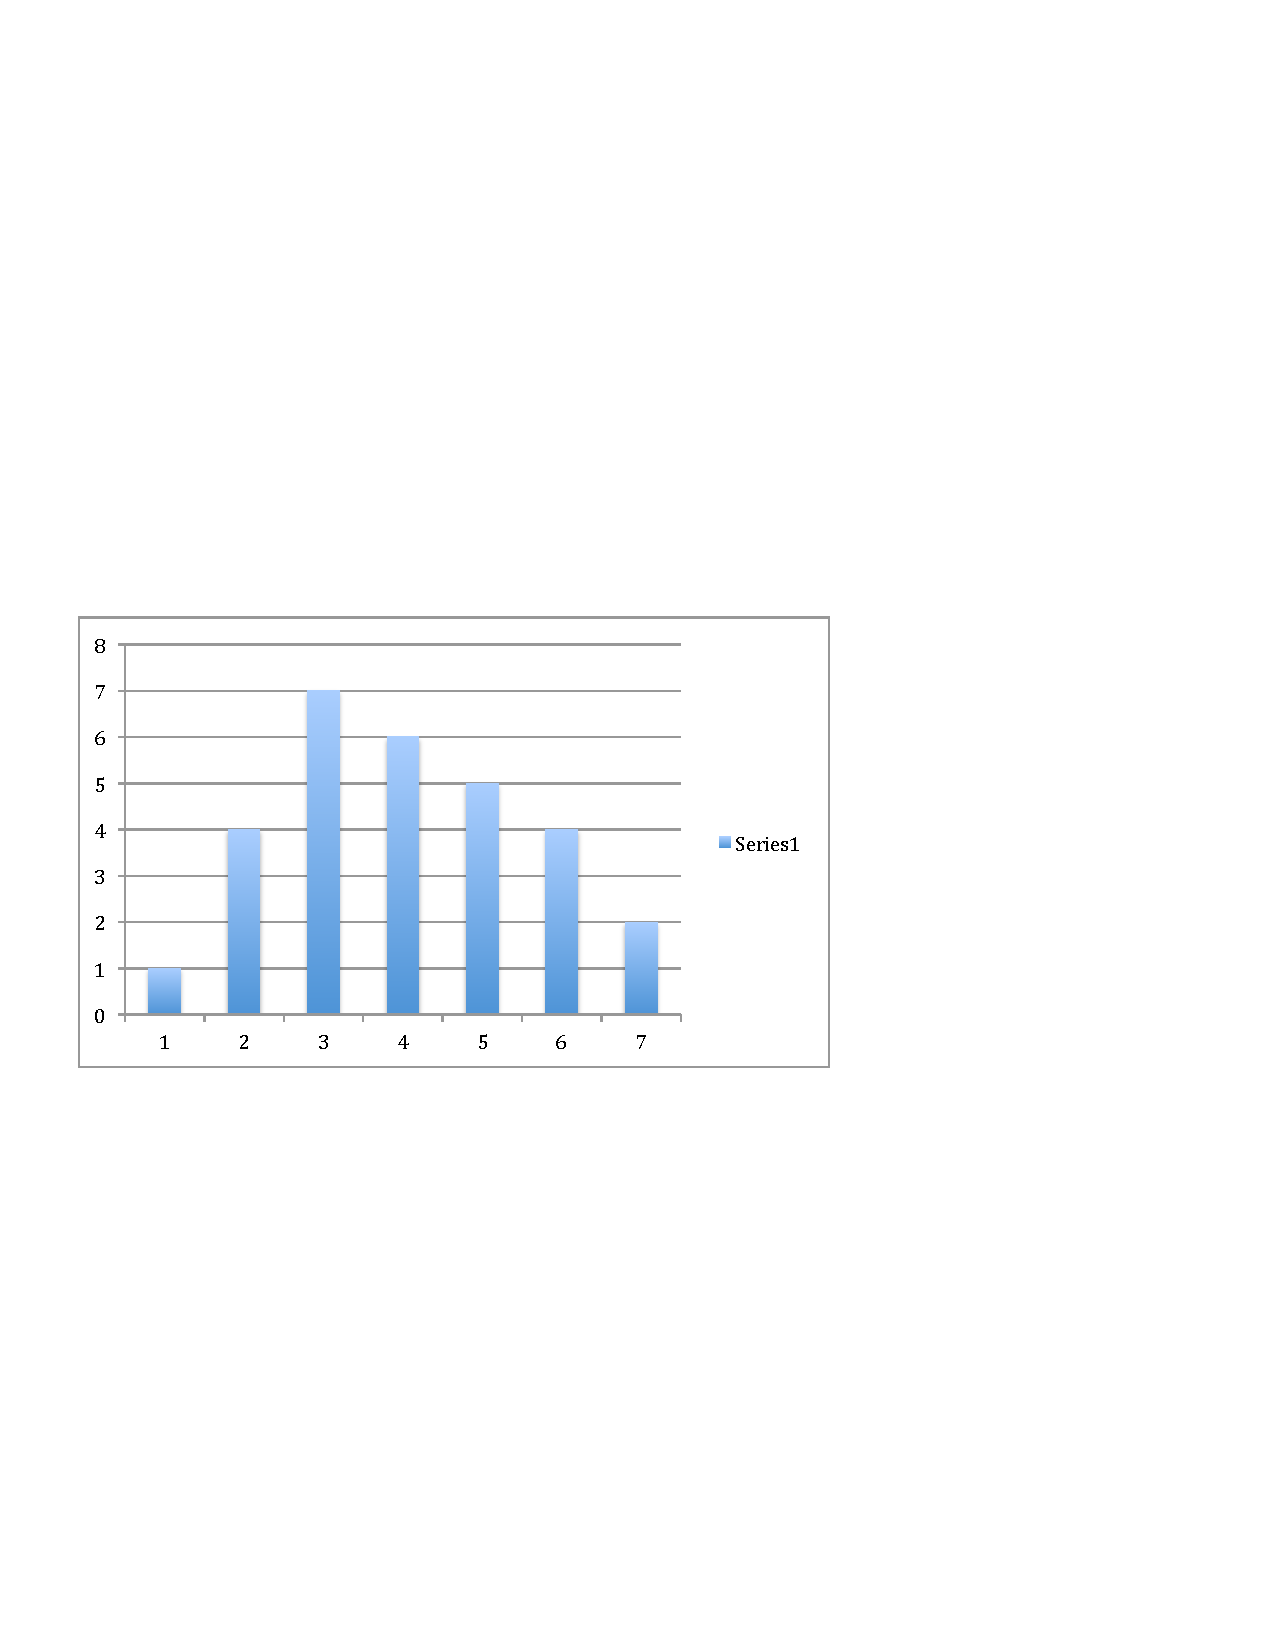
\includegraphics[width=.7\linewidth]{LabmanualFigures/Excel15.pdf}
      \caption{A figure for the histogram}
      \label{fig:excel15}
\end{figure}
 



\subsection{Paired Samples T-test} 
Suppose you ran an experiment with one independent variable that has 2 levels. You used a within- subject design so each participant contributed data to each of the 2 levels. You want to find out if there was significant effect. That is, is the mean performance in Level 1 different from mean performance in Level 2. An appropriate test is the paired-samples t-test.
Here is some sample data in Excel.
 and the number 1 tells excel to use a paired samples t-test. The resulting p-value is <.05 so we now know that there was a significant effect. The means for level 1 were significantly smaller than the means for level 2.

\begin{figure}
      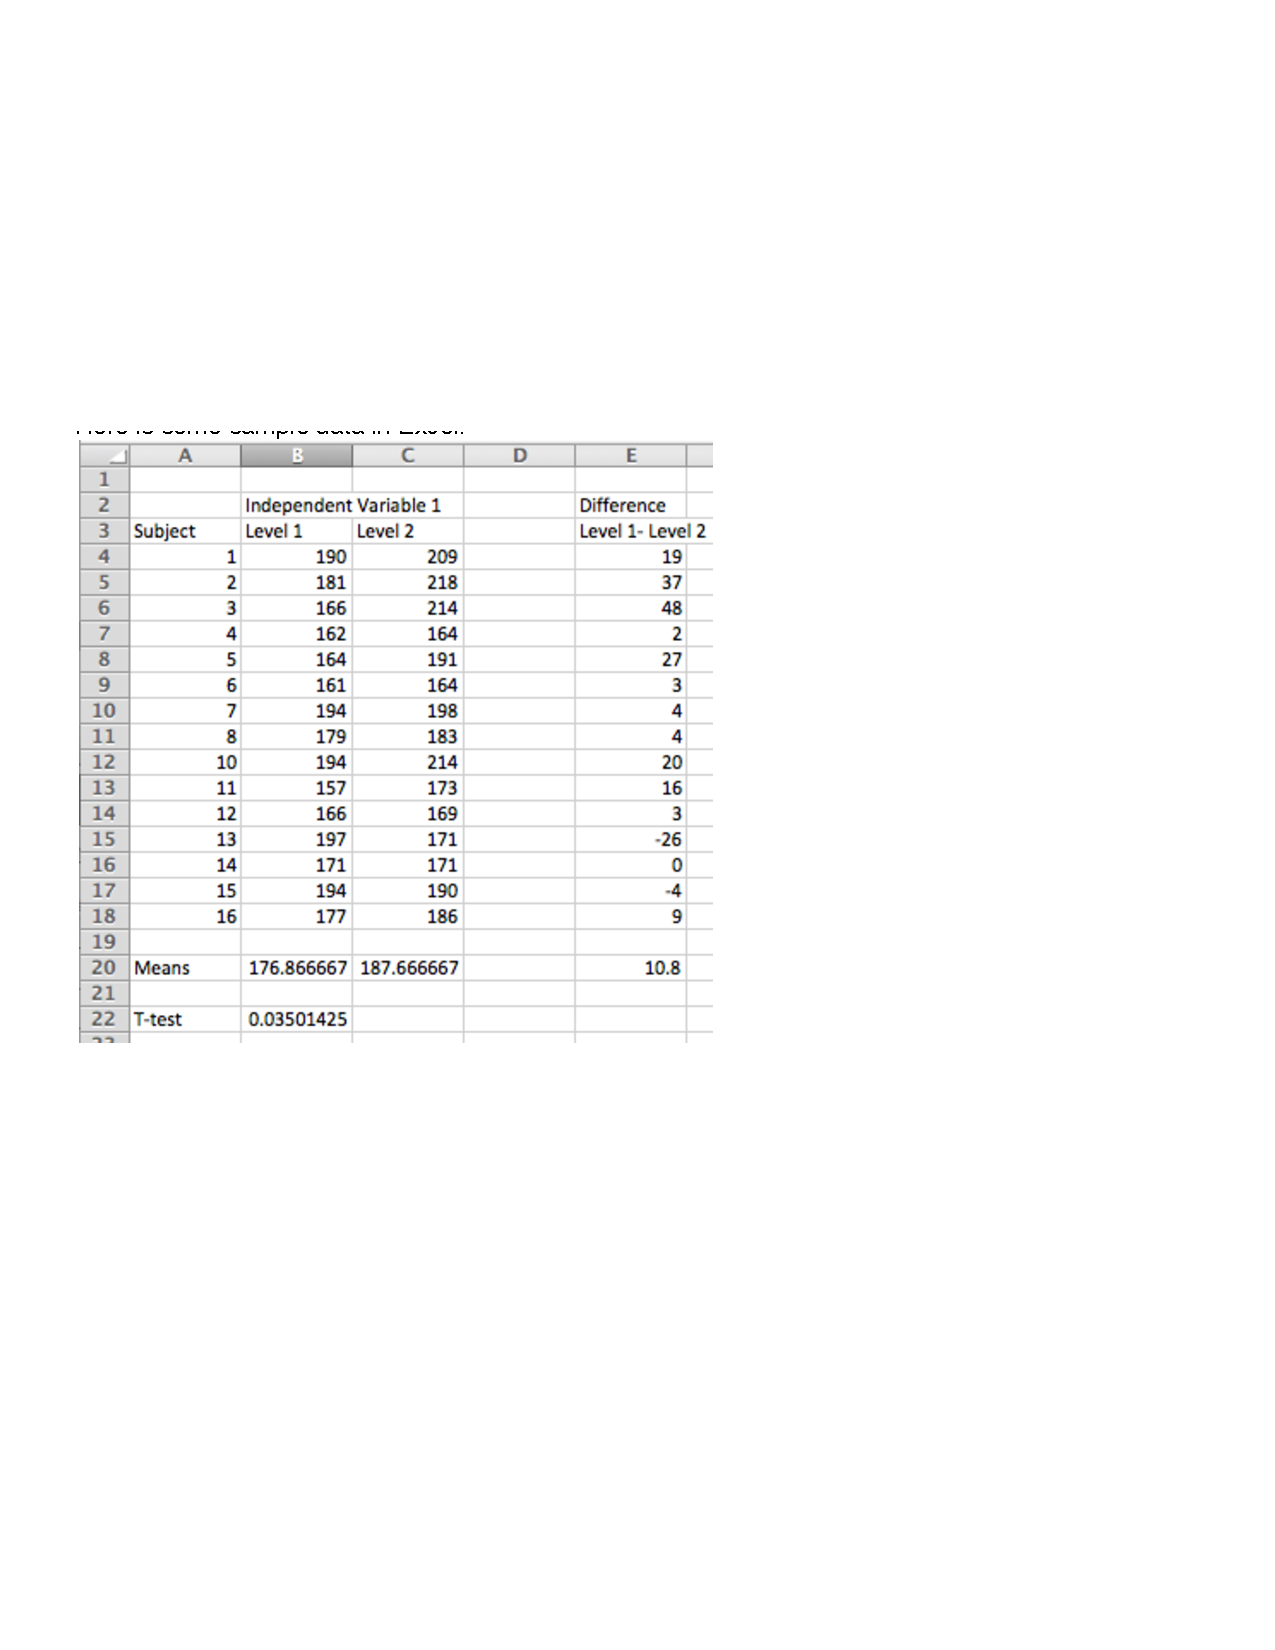
\includegraphics[width=.7\linewidth]{LabmanualFigures/Excel16.pdf}
      \caption{t test in excel}
      \label{fig:excel16}
\end{figure}
 


Tip: Even before you run a paired samples t-test you should have a good idea whether the test will be significant. You can get a ballpark estimate by computing the differences between means for each subject. This has been done in the example under the column labeled Difference. Here, the mean for level 1 has been subtracted from the mean for level 2 for each subject. This gives us a difference score. Look at all of the difference scores. You will see that almost all of them (except for 2) are positive. So, most of the subjects showed the effect. As a ballpark rule, when most of the subjects show the effect you should expect that a t-test will likely show a significant result.

\section{SPSS}

\subsection{Paired Samples T-test in SPSS} 

\begin{figure}
      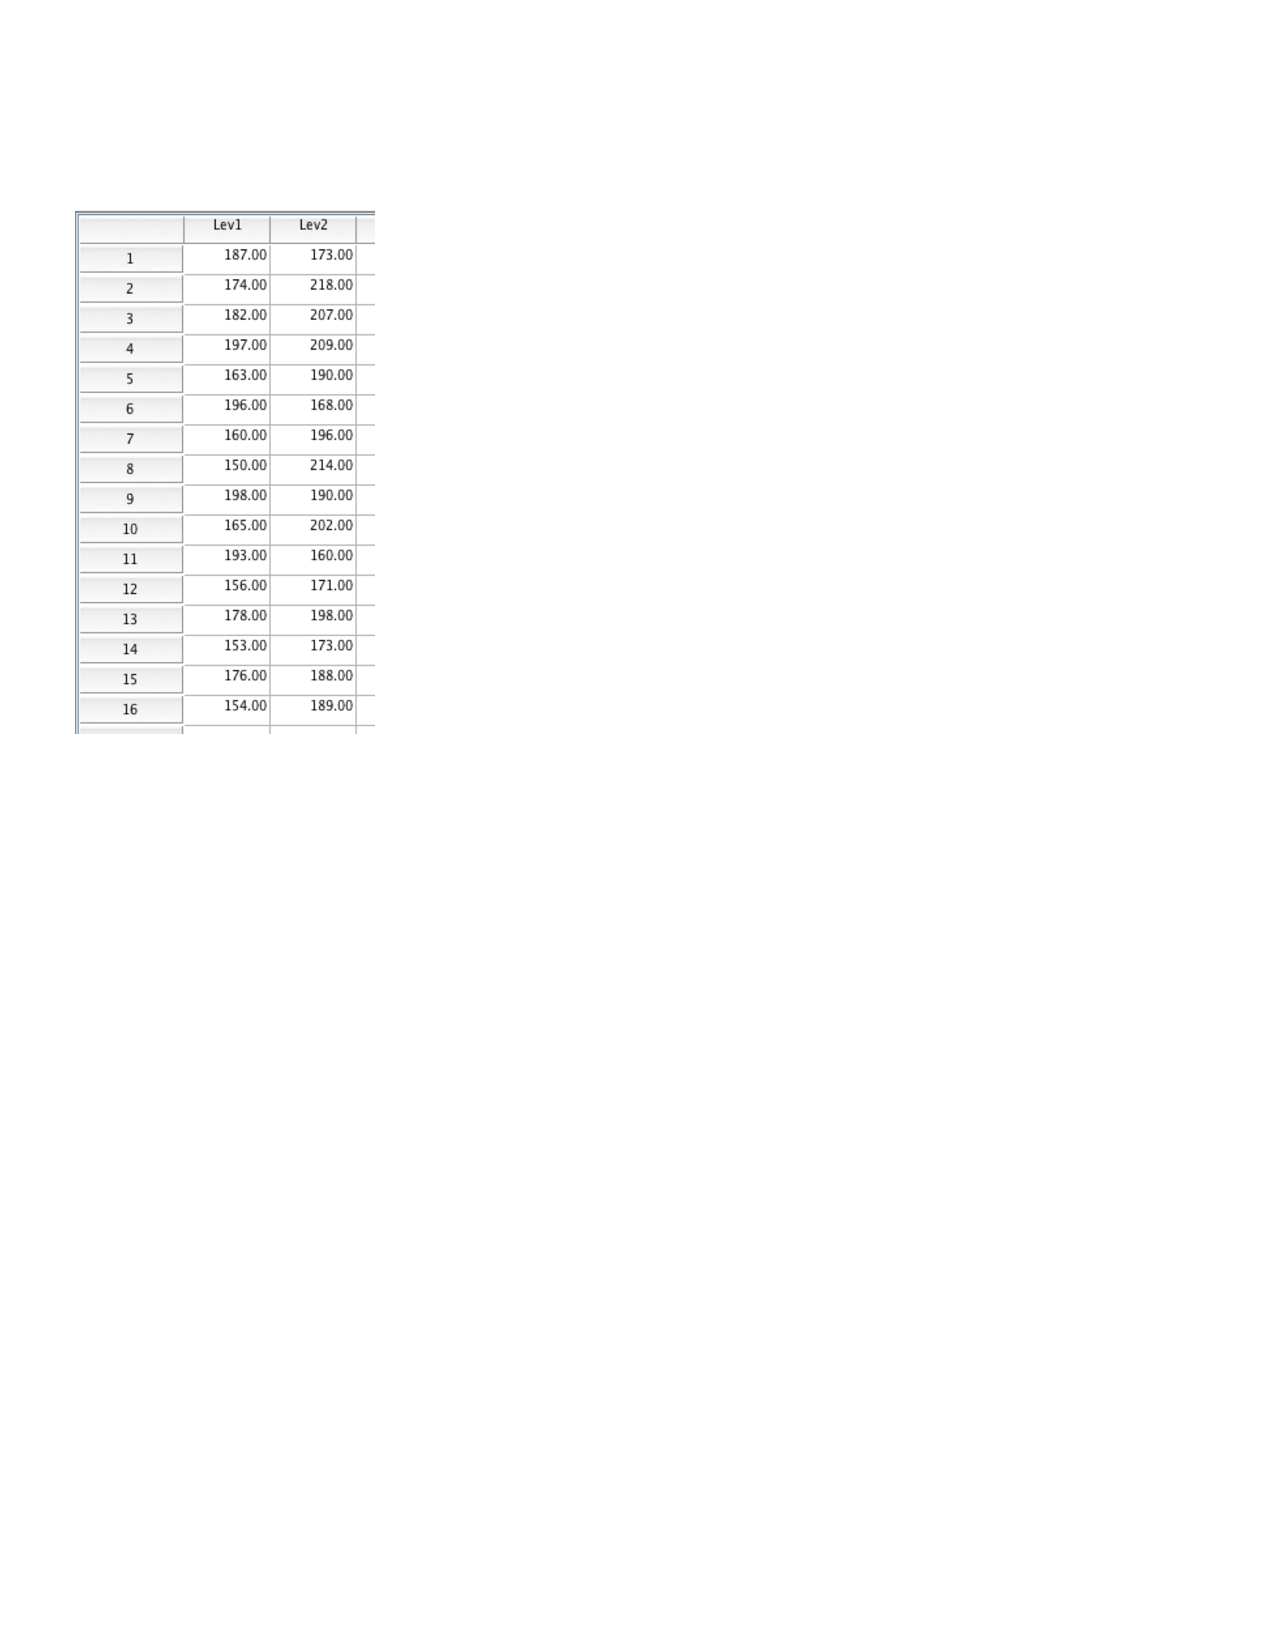
\includegraphics[width=.5\linewidth]{LabmanualFigures/SPSS1.pdf}
      \caption{Copy the data into SPSS}
      \label{fig:spss1}
\end{figure}

1. Copy the data for each level of the independent variable into separate columns in the data editor. In the example I've given new names (lev1, lev2) to each of the conditions.


\begin{figure}
      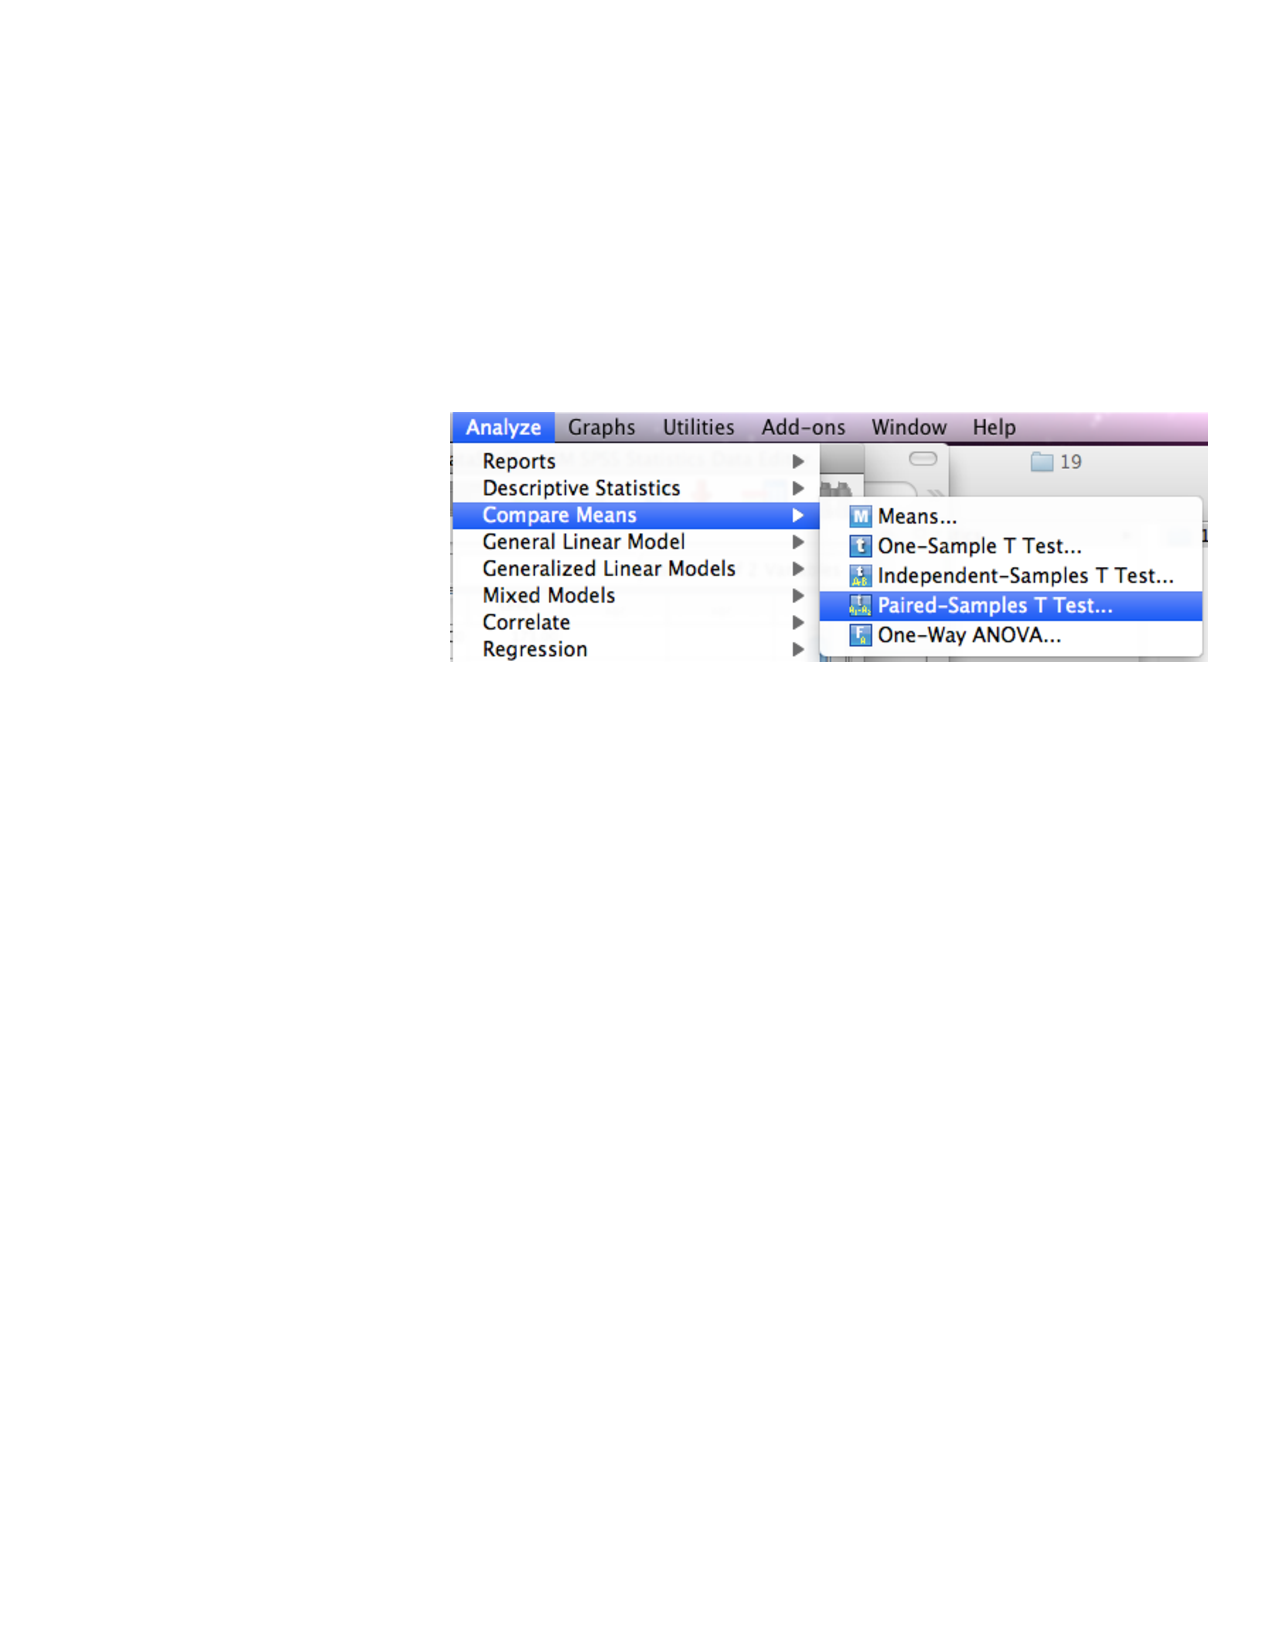
\includegraphics[width=.5\linewidth]{LabmanualFigures/SPSS2.pdf}
      \caption{Choose t-test}
      \label{fig:SPSS2}
\end{figure}

2. Next,choose analyze from the menu, select Compare Means, then select Paired-Samples T Test


3. You will see the following menu. Select both of your variables (Lev1, Lev2) then press the arrow button to move them into the paired variables list
   

\begin{figure}
      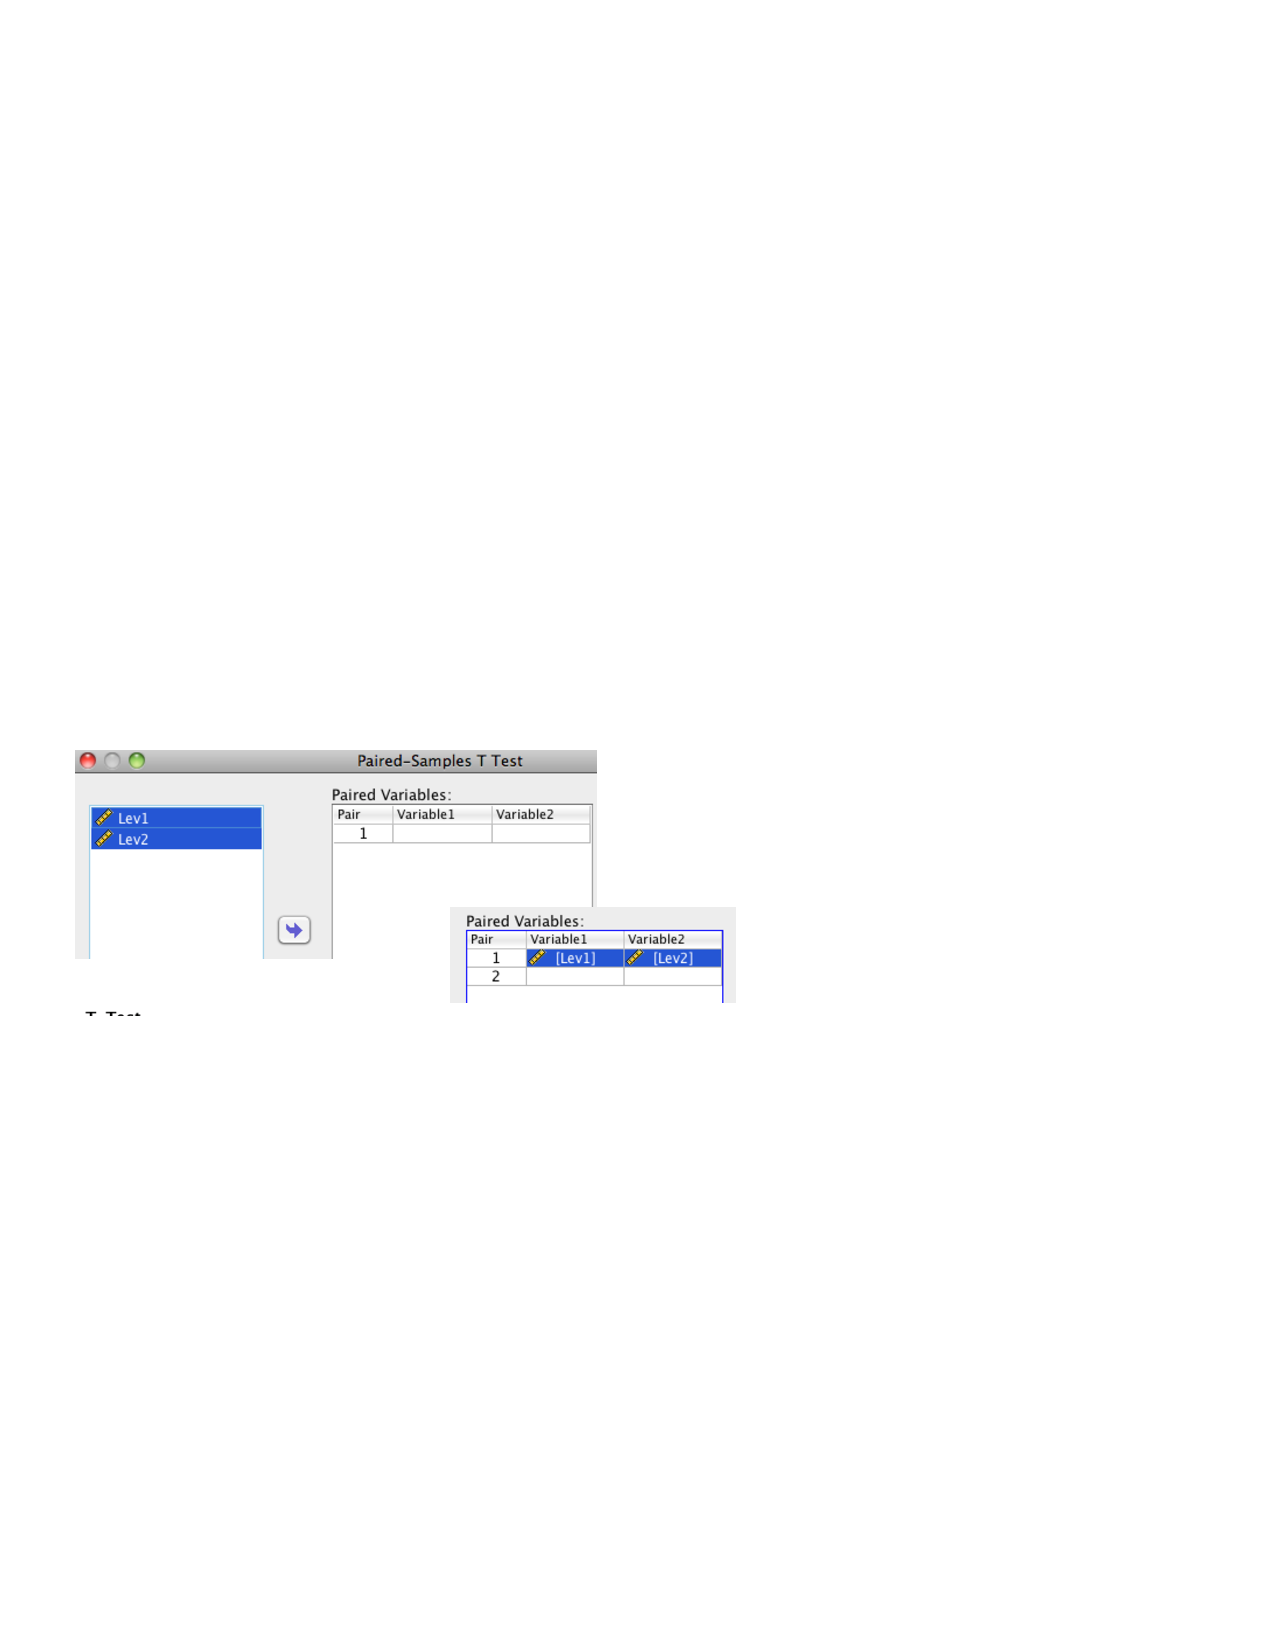
\includegraphics[width=.5\linewidth]{LabmanualFigures/SPSS3.pdf}
      \caption{Select levels}
      \label{fig:SPSS3}
\end{figure}

4. It should look like this... now click the button for the analysis


5. The first box shows basic descriptive statistics, means, number per cell, standard deviation and standard error of the mean.


\begin{figure}
      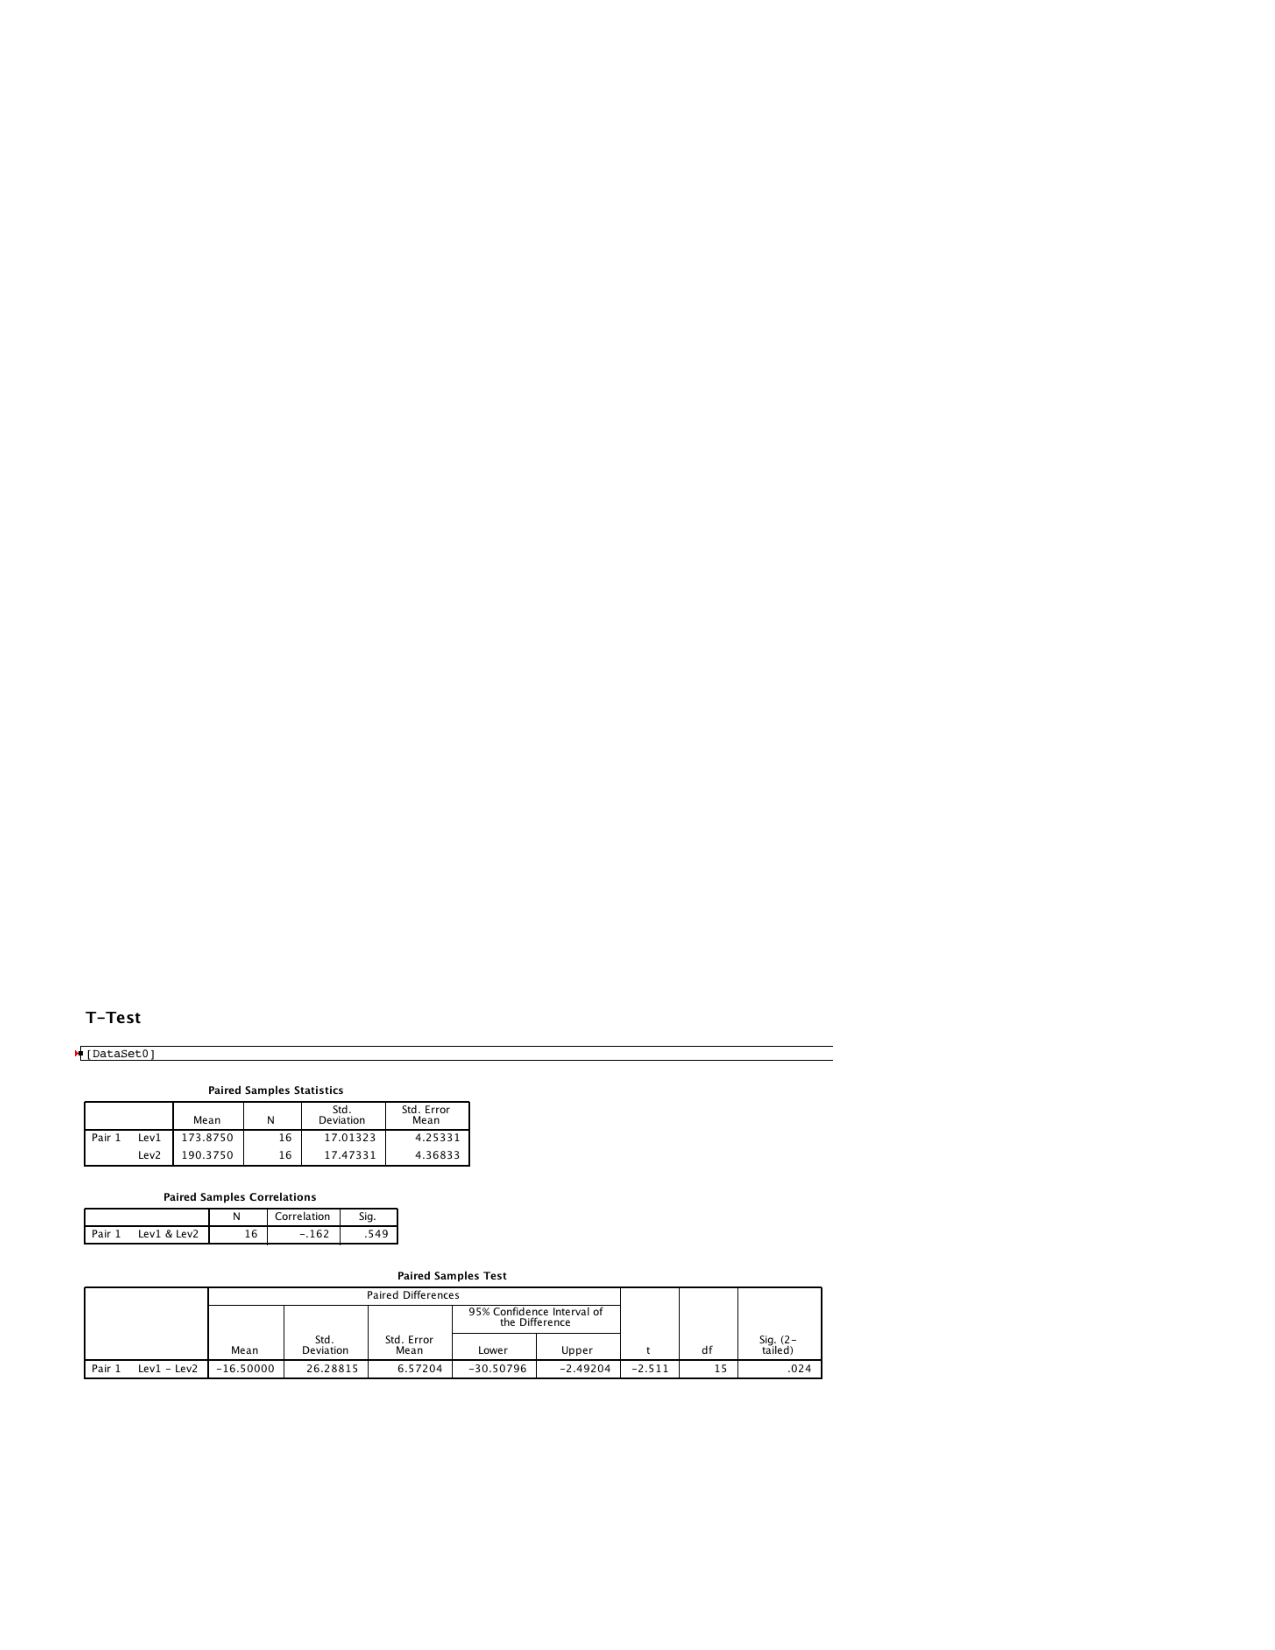
\includegraphics[width=\linewidth]{LabmanualFigures/SPSS4.pdf}
      \caption{ttest output}
      \label{fig:SPSS4}
\end{figure}

6. The third box shows the t-value, the associated degrees of freedom (df), and the p- value (Sig. (2-tailed)


7. Here's how you write up your results in one sentence.


8. Means were significantly smaller for level 1 (174) than level 2 (190), t(15) = 2.51, p<.05.
  
\subsection{2 x 2 Repeated Measures ANOVA}
\subsection{From Data to Analysis}

Suppose you ran an experiment with 2 independent variables, each with 2 levels. If this is a within- subject design, each participant will contribute data to each of the 4 levels in the design. The appropriate test is a 2x2 repeated measures ANOVA. We begin by looking at the data in excel.


\begin{figure}
      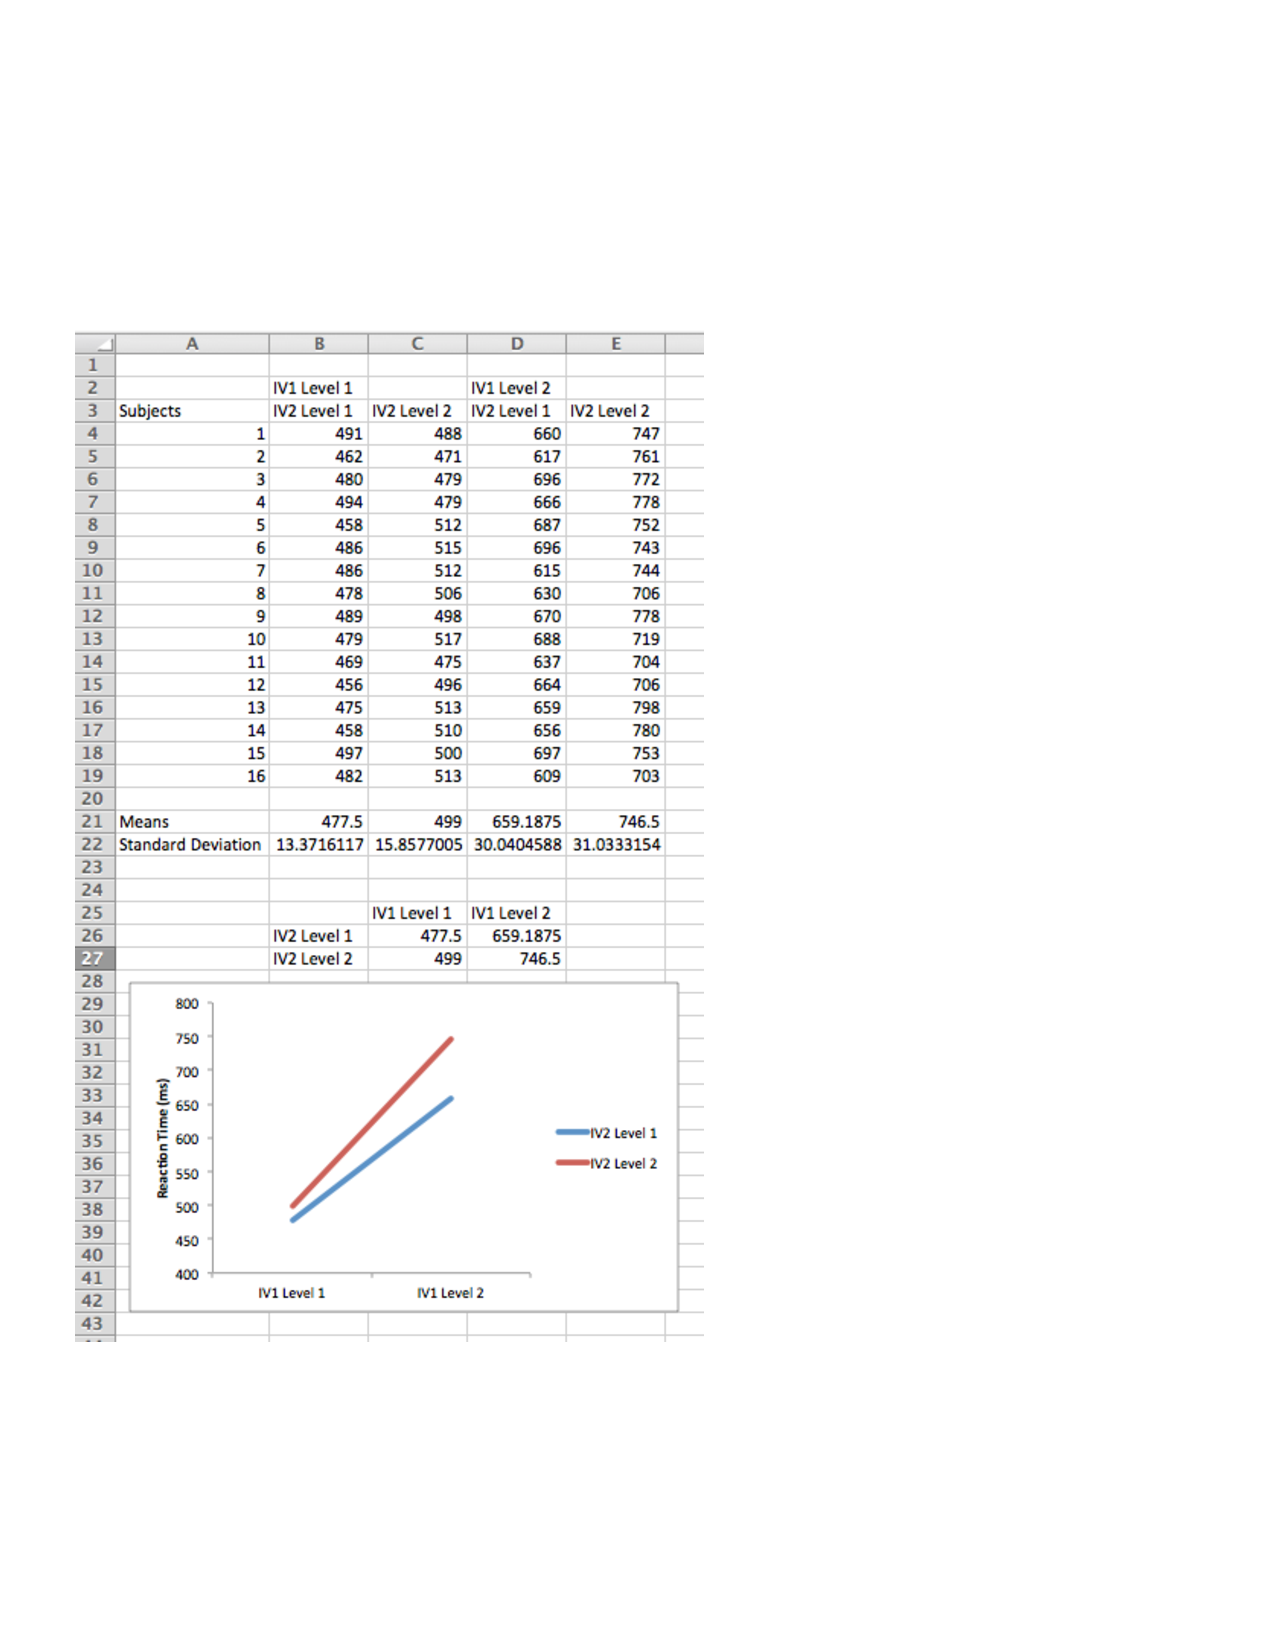
\includegraphics[width=.7\linewidth]{LabmanualFigures/SPSS5.pdf}
      \caption{Sample data for a 2 x 2 factorial design}
      \label{fig:SPSS5}
\end{figure}

1. All of the four conditions are placed into 4 separate columns. The second IV is nested underneath the first IV.

2. The means and standard deviations can be computed directly in excel for each of the conditions

3. The means are then organized in a table, and a figure can be created so that we can see the pattern of results.

4. Main effects: It looks like there are two main effects. One for IV1: level 1 is smaller than level 2. One for IV2: level 1 is smaller than level 2

5. Interaction:It looks like there is an interaction. The difference between L1 and L2 of IV1 is larger for level 1 of IV2 (in red) than level 2 of IV2 (in blue).

6. We need to run a 2x2 repeated
measures ANOVA to determine whether the main effects are significant, and to determine if the interaction is significant.


\subsection{2x2 Repeated measures ANOVA in SPSS}
 
\begin{figure}
      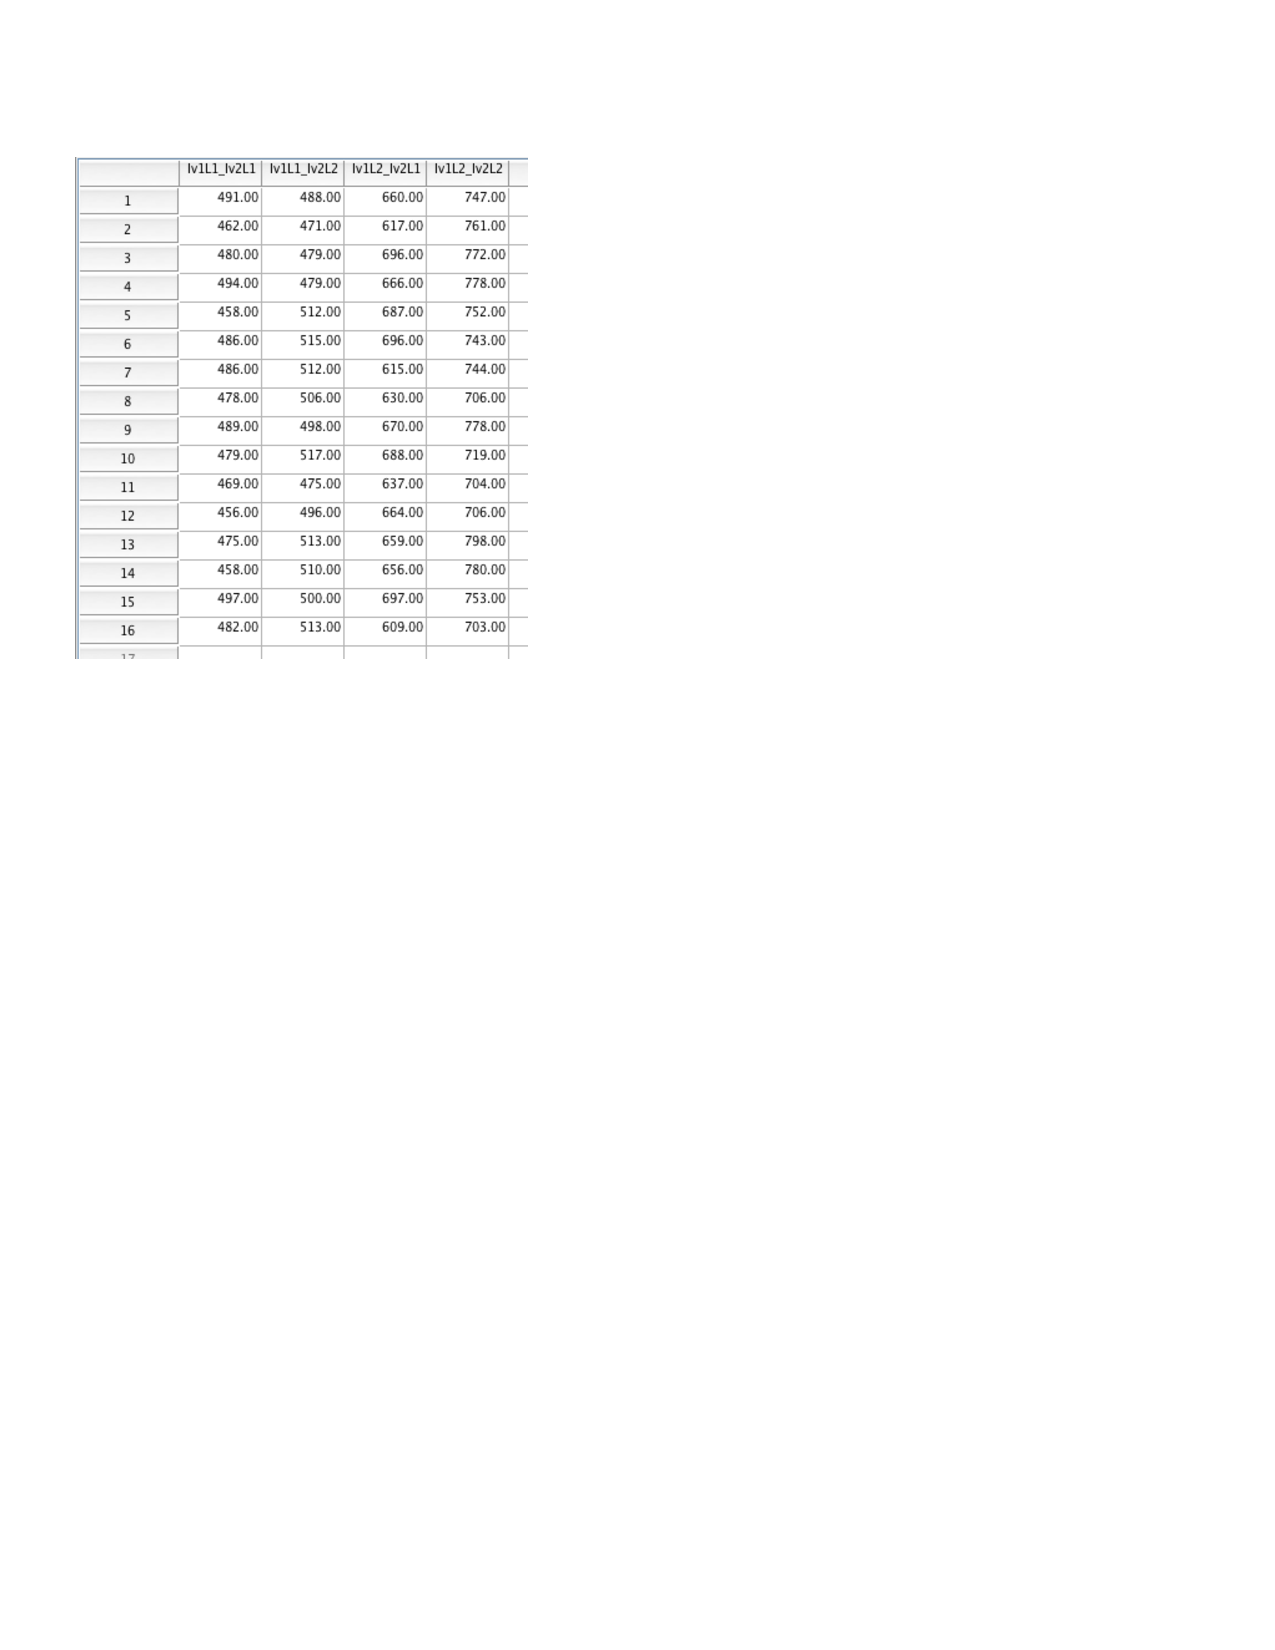
\includegraphics[width=.6\linewidth]{LabmanualFigures/SPSS6.pdf}
      \caption{Copy data into SPSS}
      \label{fig:SPSS6}
\end{figure}

1. Copy the data into SPSS. Make sure each column represents a different condition in the design.

2. Give names to each of the variables. The first column represents IV1 Level1 \& IV2 Level 1. The second column represents IV1 Level 1 \& IV2 Level 2. The third column represents IV1 Level 2 \& IV2 Level 1. The fourth column represents IV1 Level 2 \& IV2 Level 2.

\begin{figure}
      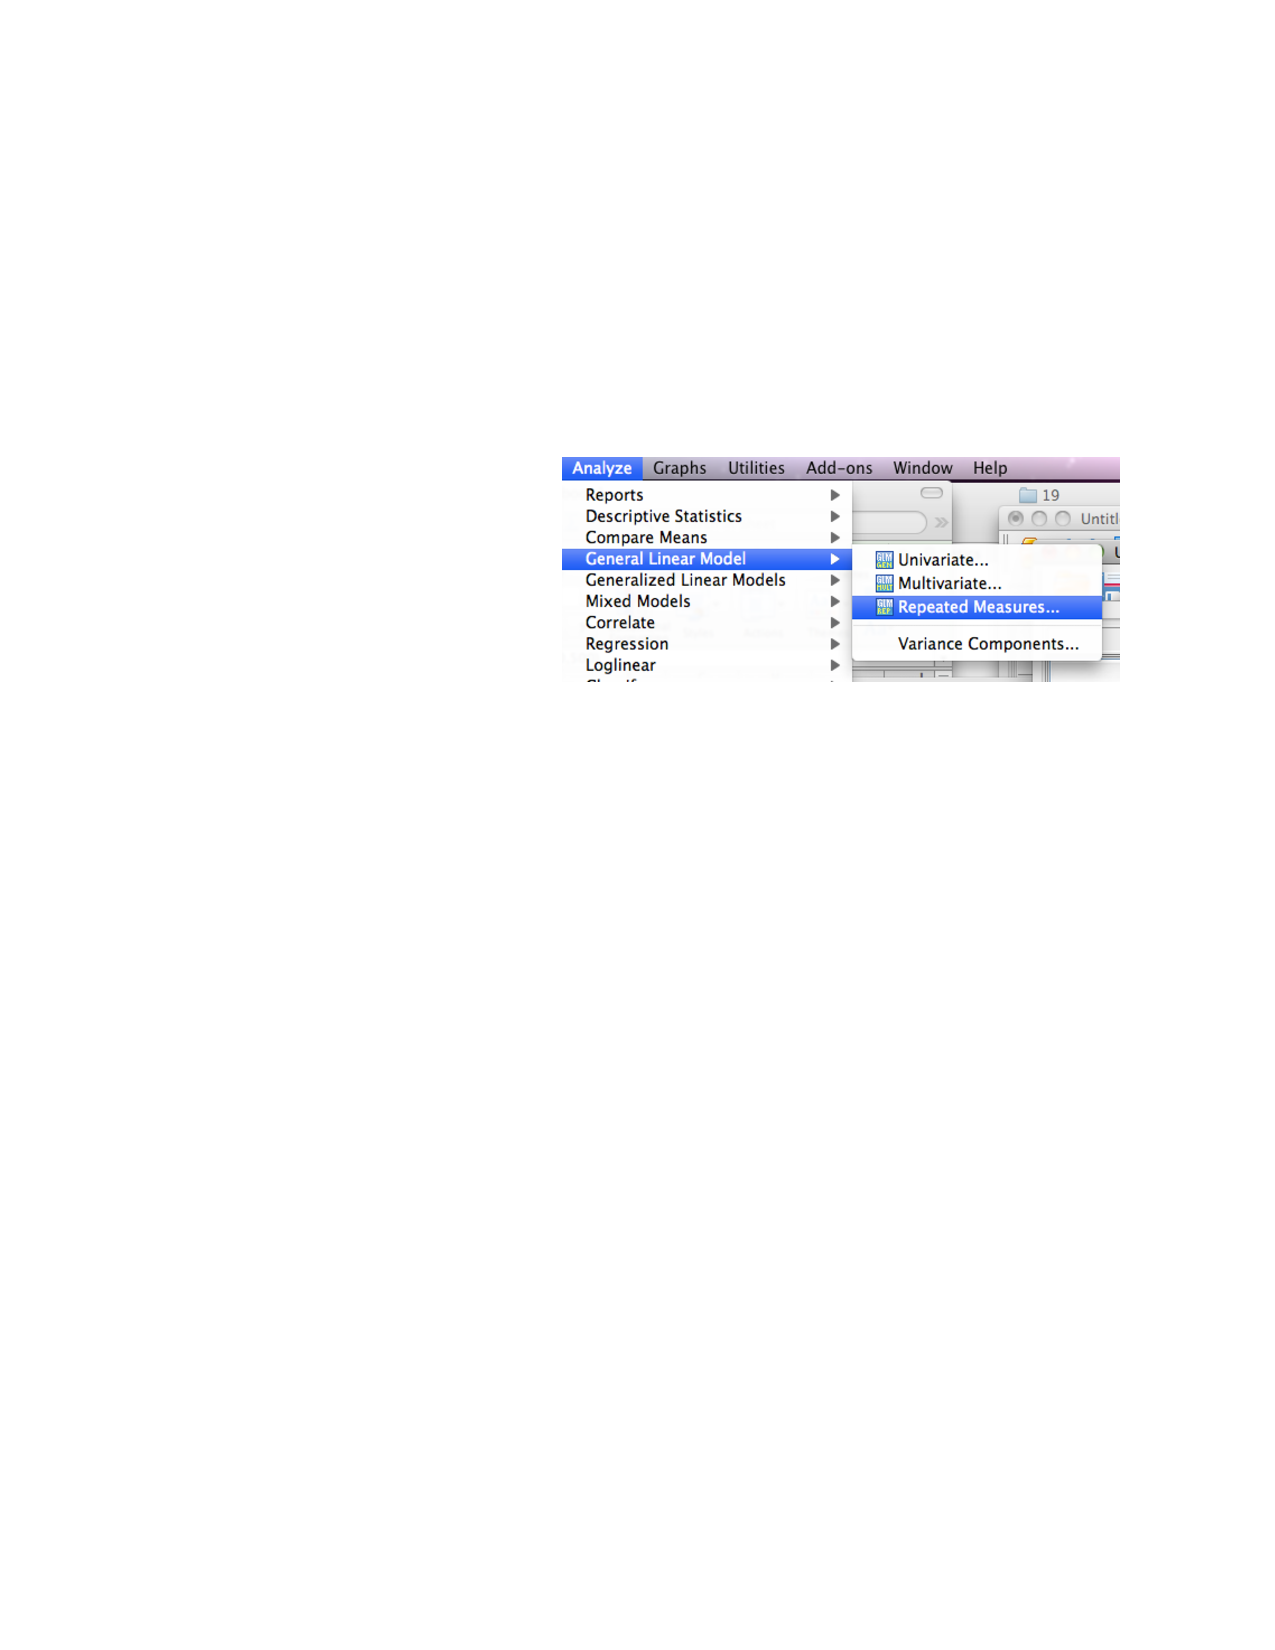
\includegraphics[width=.5\linewidth]{LabmanualFigures/SPSS7.pdf}
      \caption{Choose the model}
 	\label{fig:sp7}
\end{figure}

3. Choose Analyze, General Linear Model, Repeated Measures from the menu.
   
\begin{figure}
      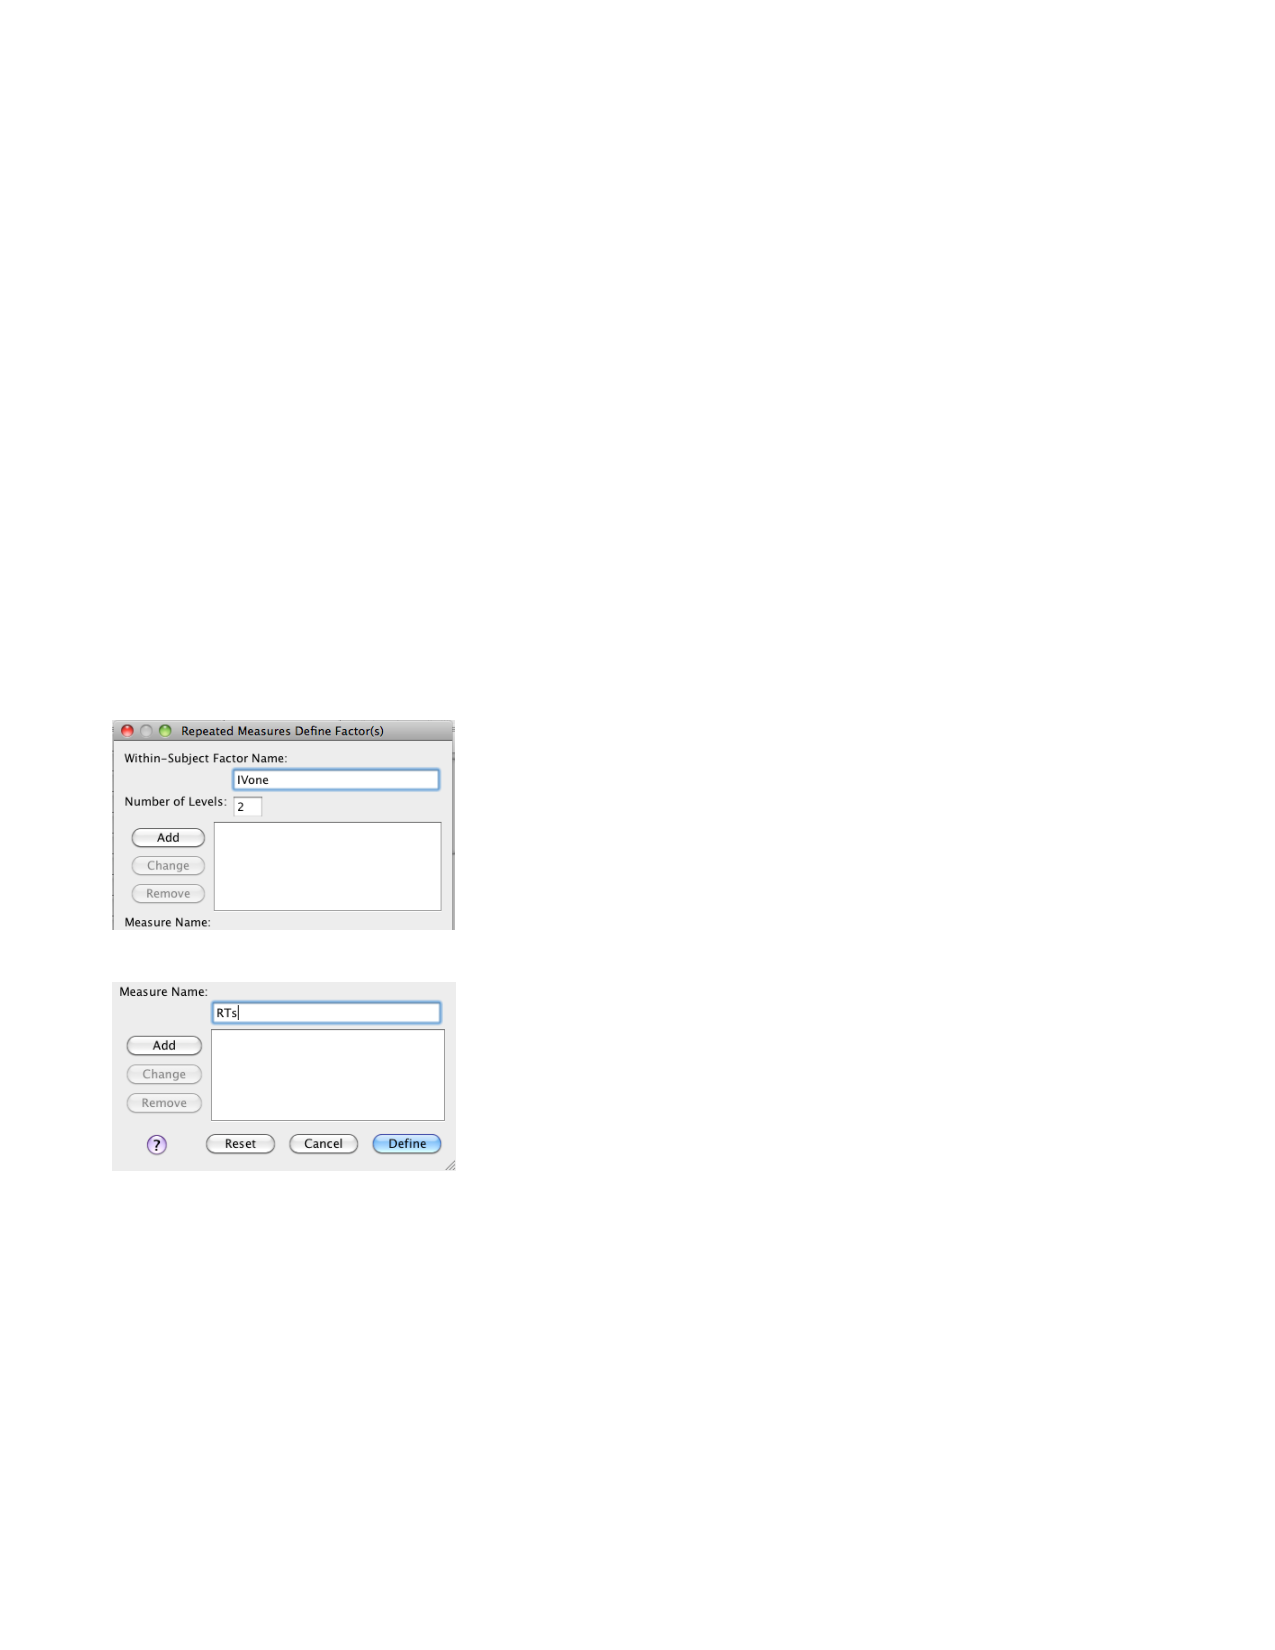
\includegraphics[width=.5\linewidth]{LabmanualFigures/SPSS8.pdf}
      \caption{Name variables}
      \label{fig:SPSS8}
\end{figure}

\begin{figure}
      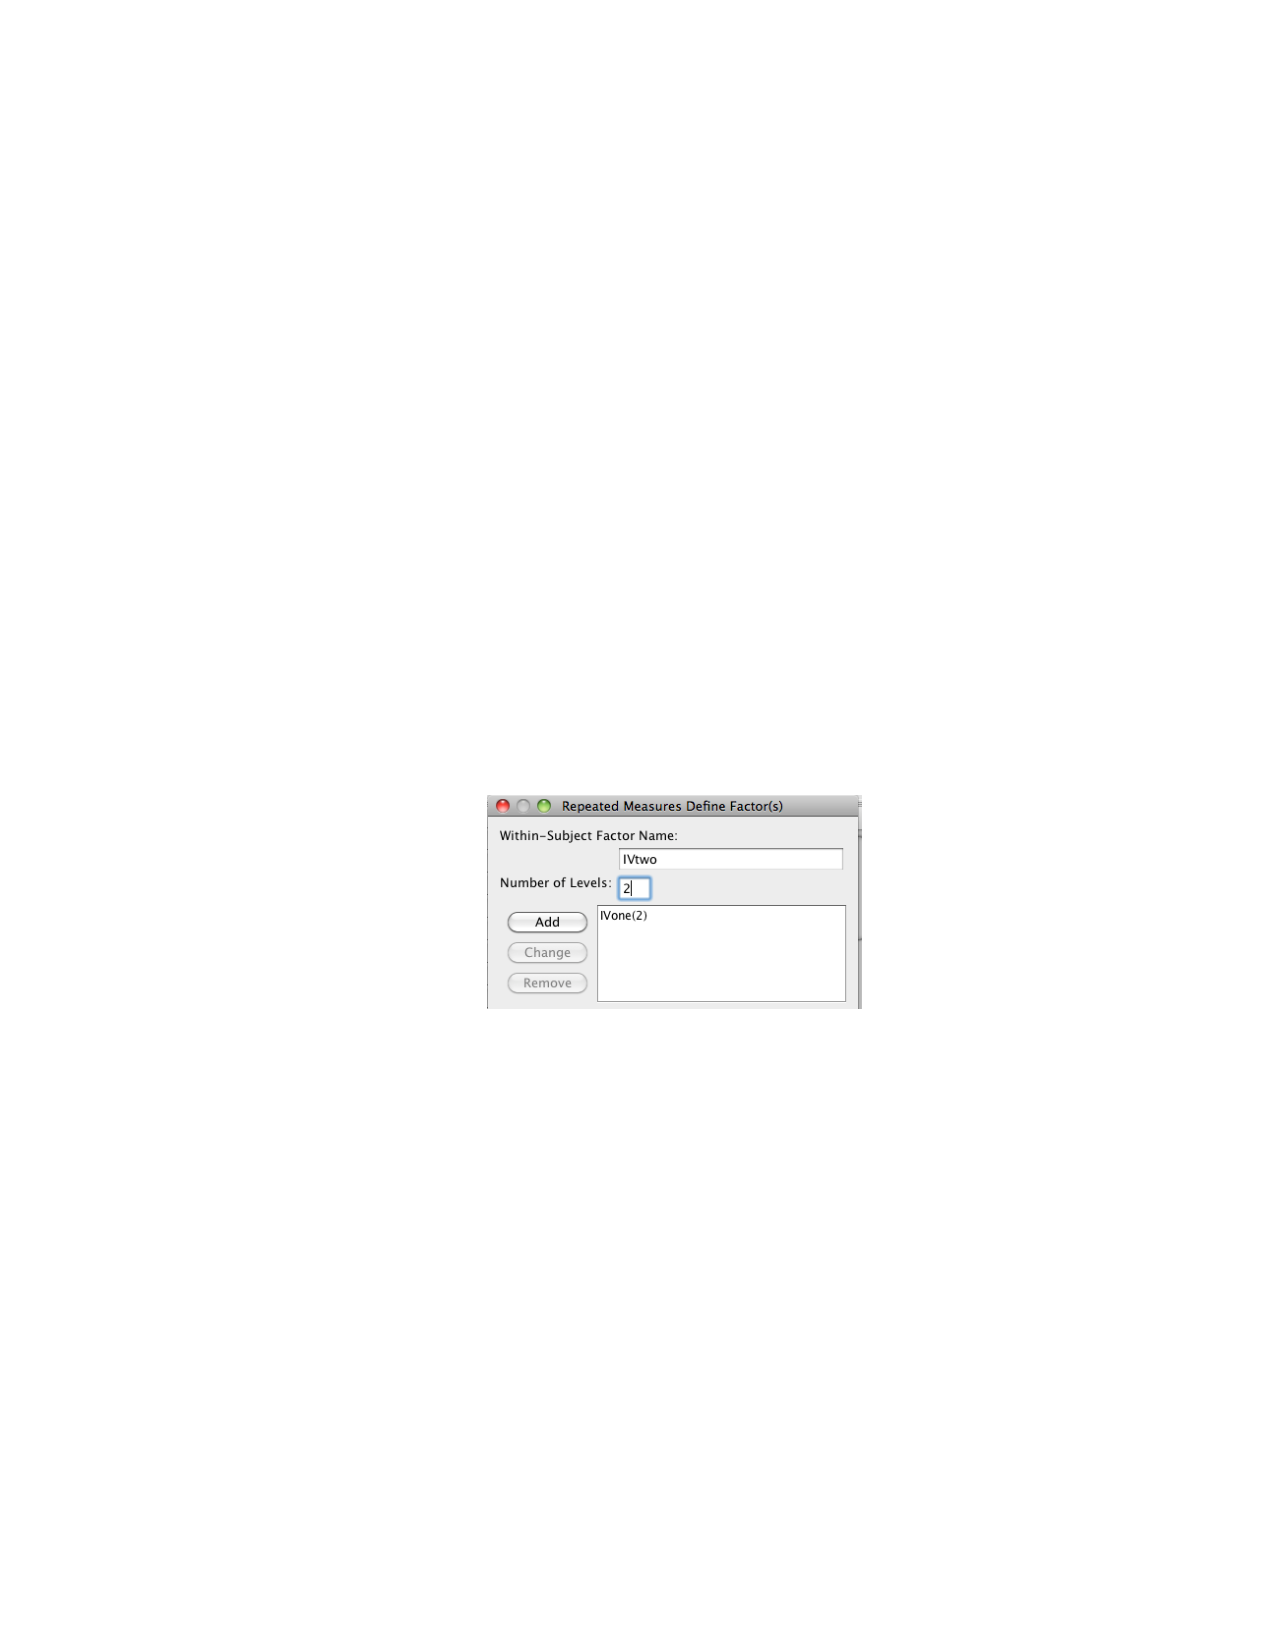
\includegraphics[width=.5\linewidth]{LabmanualFigures/SPSS9.pdf}
      \caption{ thing a}
      \label{fig:SPSS9}
\end{figure}

4. Name IV1, specify 2 levels

5. Name IV1, specify 2 levels

6. Name dependent variable, click define

7. Select all four conditions, press the first right arrow, if you want more options see below, otherwise press ok.

\begin{figure}
      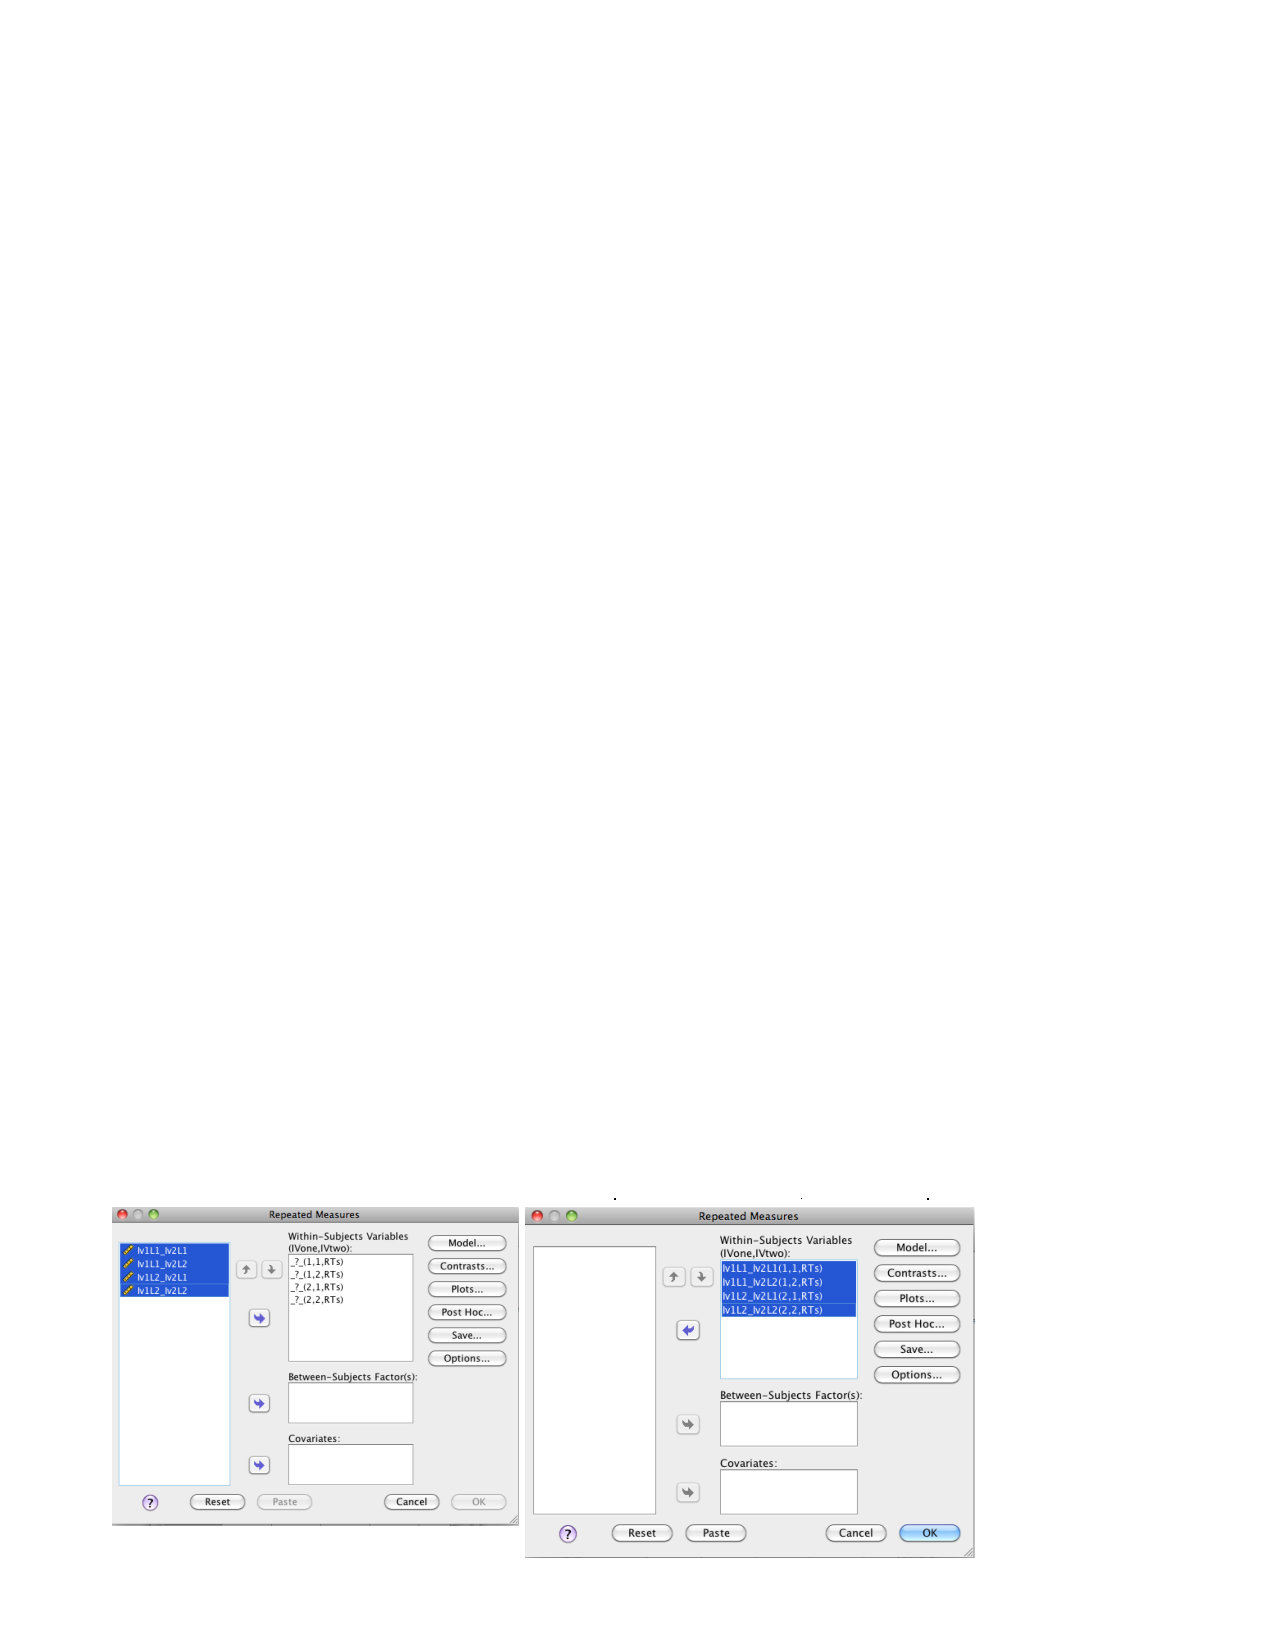
\includegraphics[width=\linewidth]{LabmanualFigures/SPSS10.pdf}
      \caption{Select conditions}
      \label{fig:SPSS10}
\end{figure}

8. If you pressed options, then you can ask SPSS to report descriptive statistics for each condition. Choose the factors that you want, then press the arrow button to move them into the display means field. Make sure you click descriptive statistics. Then click continue.

\begin{figure}
      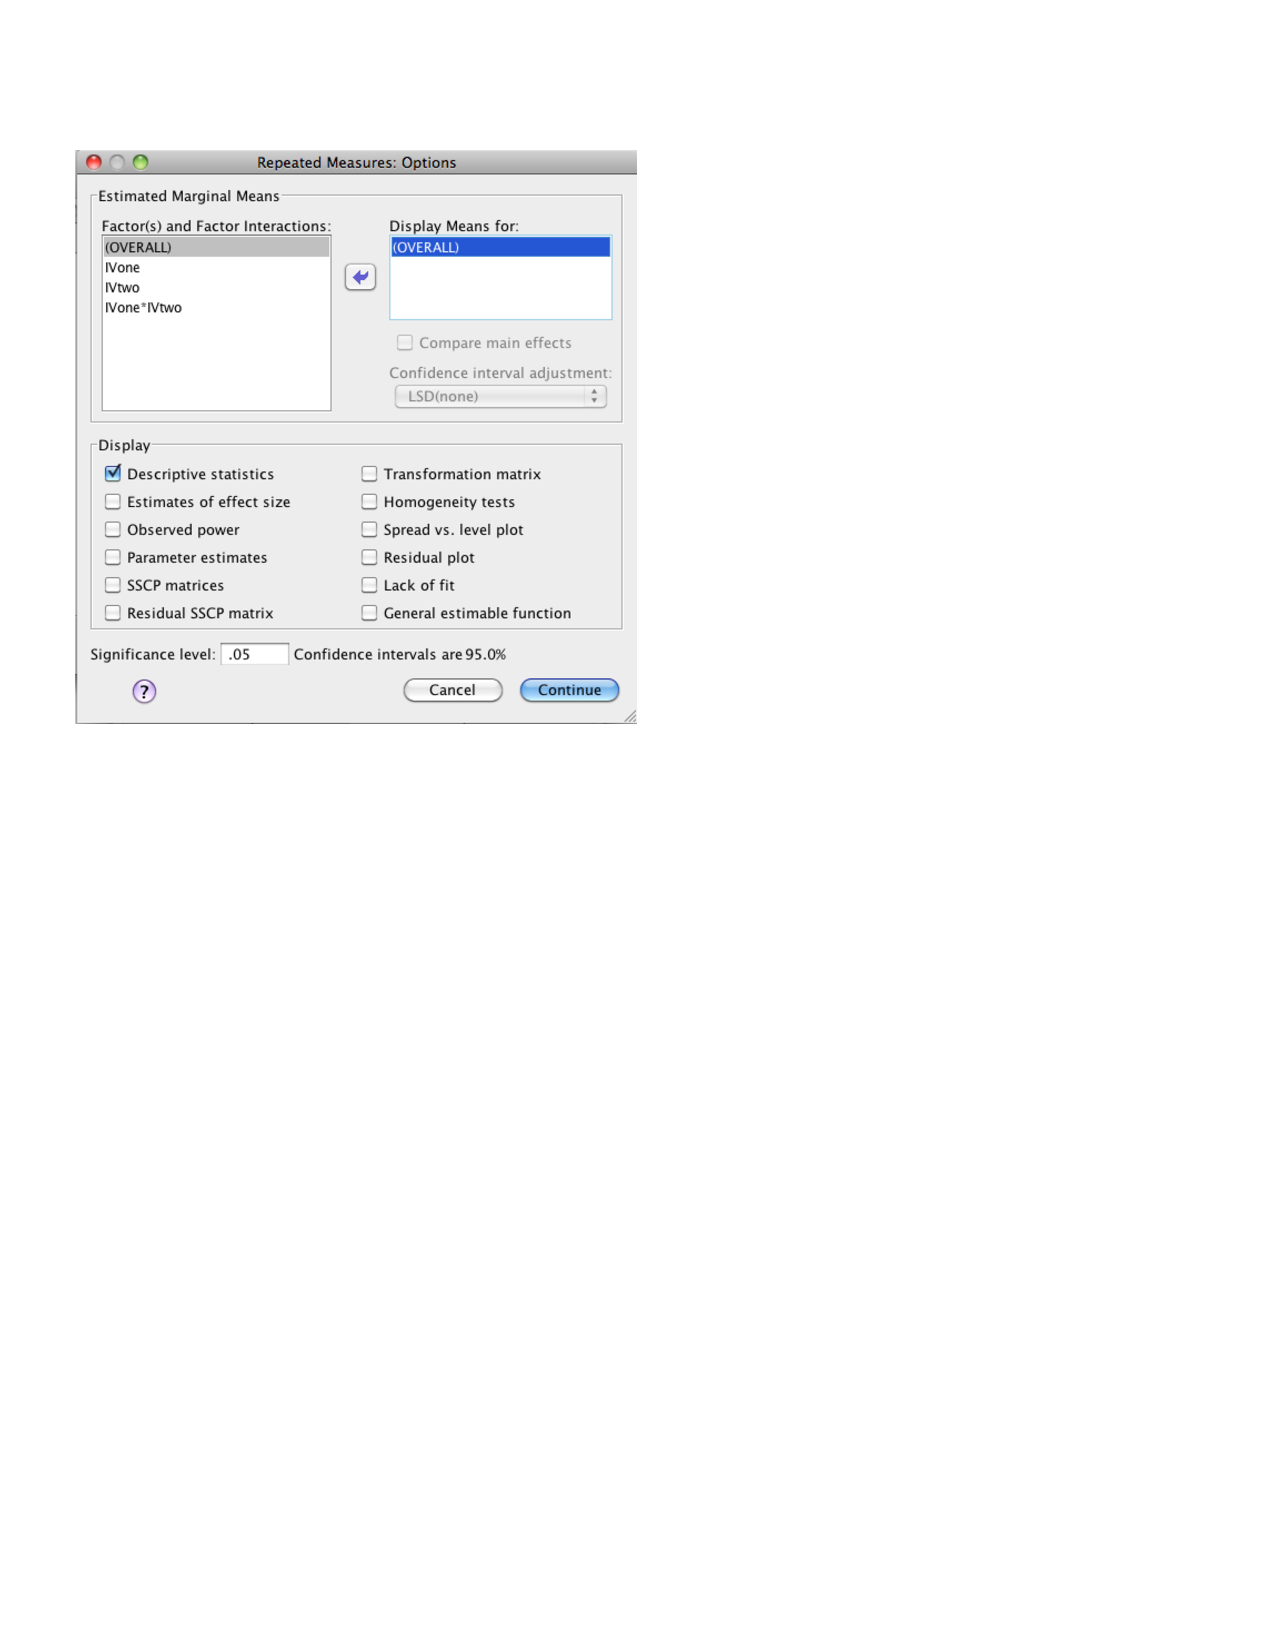
\includegraphics[width=\linewidth]{LabmanualFigures/SPSS11.pdf}
      \caption{Option to report descriptive statistics}
      \label{fig:SPSS11}
\end{figure}

\subsection{Finding numbers in the SPSS analysis output}

SPSS gives you lots of information, you need to know what you are looking for. When you report the results from a 2x2 ANOVA, you will have 2 main effects, and 1 interaction. This means you will be looking for 3 F-values, 3 MSEs (Mean squared error terms), and 3 associated p-values. You will also need to know the means for the main effects and the means for the interaction.

\begin{figure}
      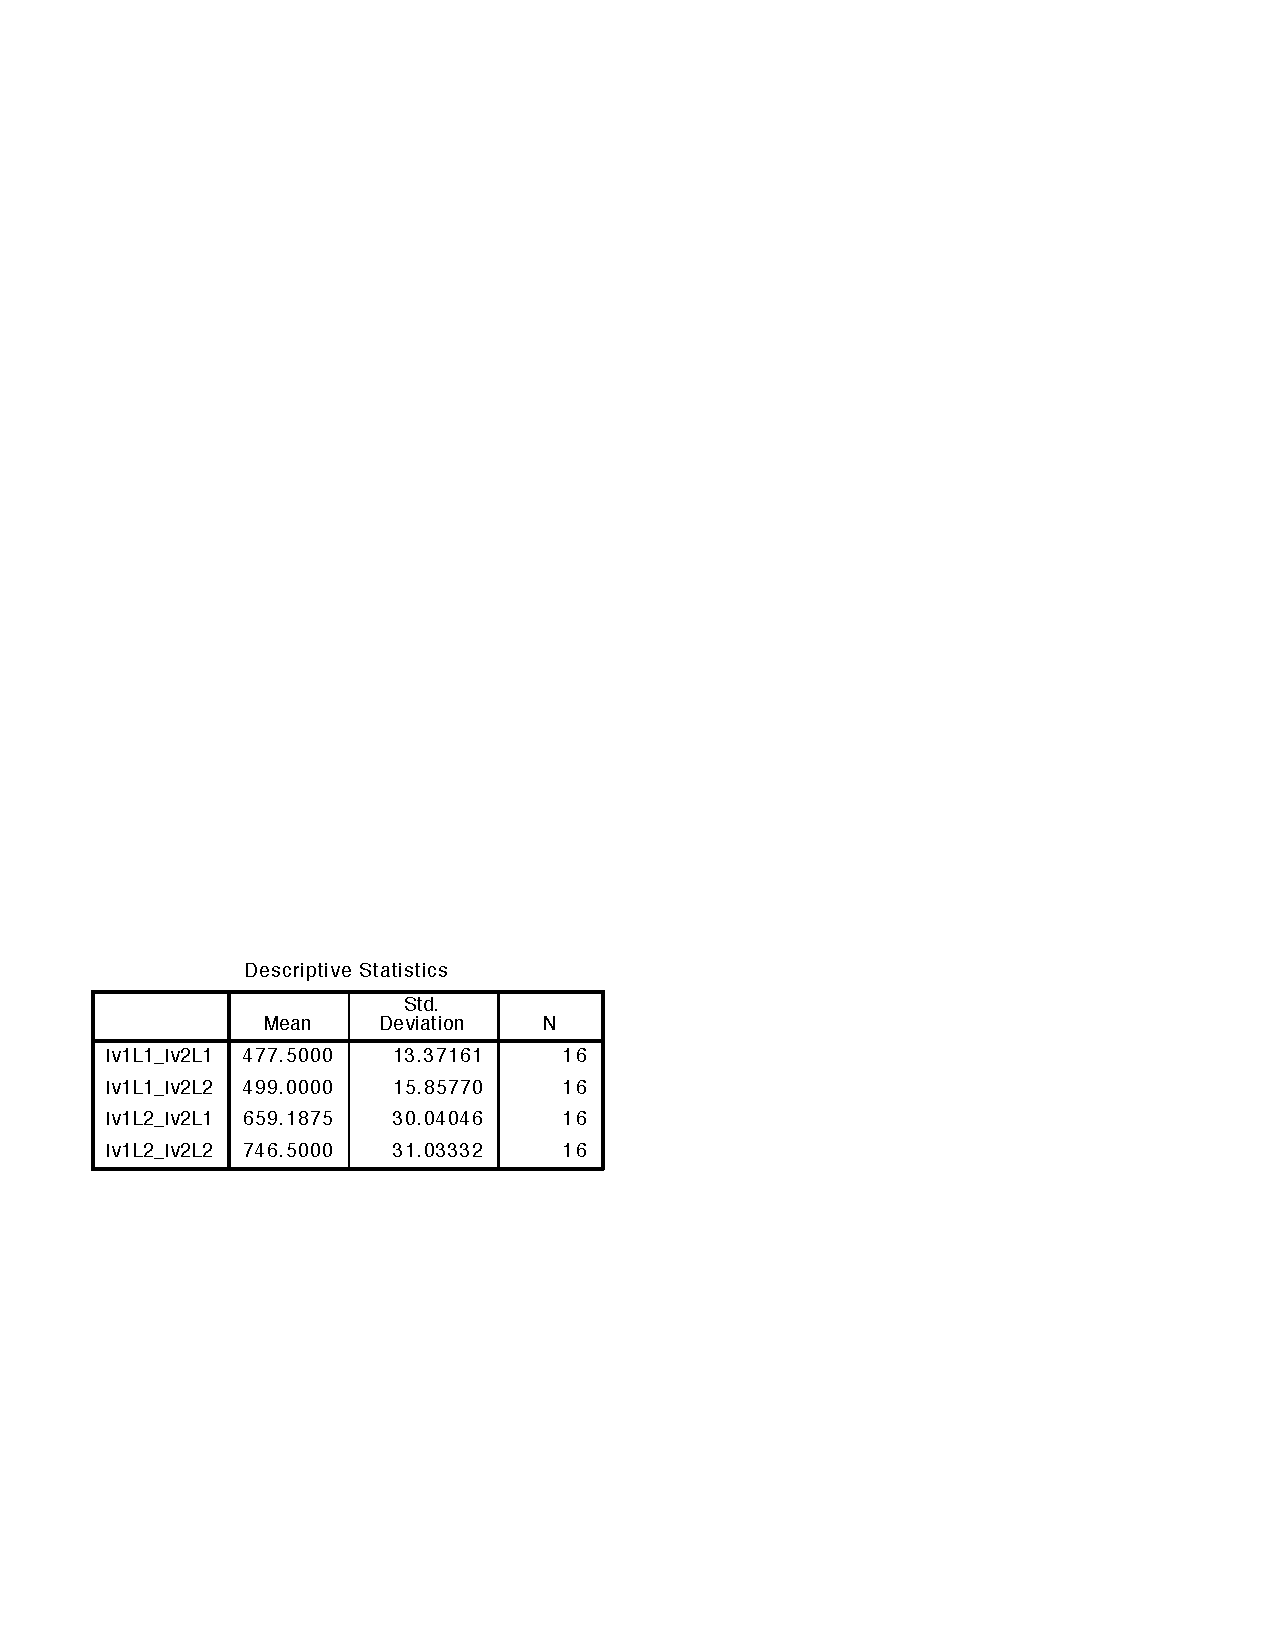
\includegraphics[width=\linewidth]{LabmanualFigures/SPSS12.pdf}
      \caption{Descriptive Statistics}
      \label{fig:SPSS12}
\end{figure}

If you chose the option for descriptive stats, then you will see a small table with Means and standard deviations for each condition in the design. You will use these means to compute averages for the main effects. You will use these means to report the pattern for the interaction.

\subsection{The ANOVA table}
All of the information that you need to report main effects and interactions is available in  the "tests of within-subjects effects" table.

\begin{figure}
      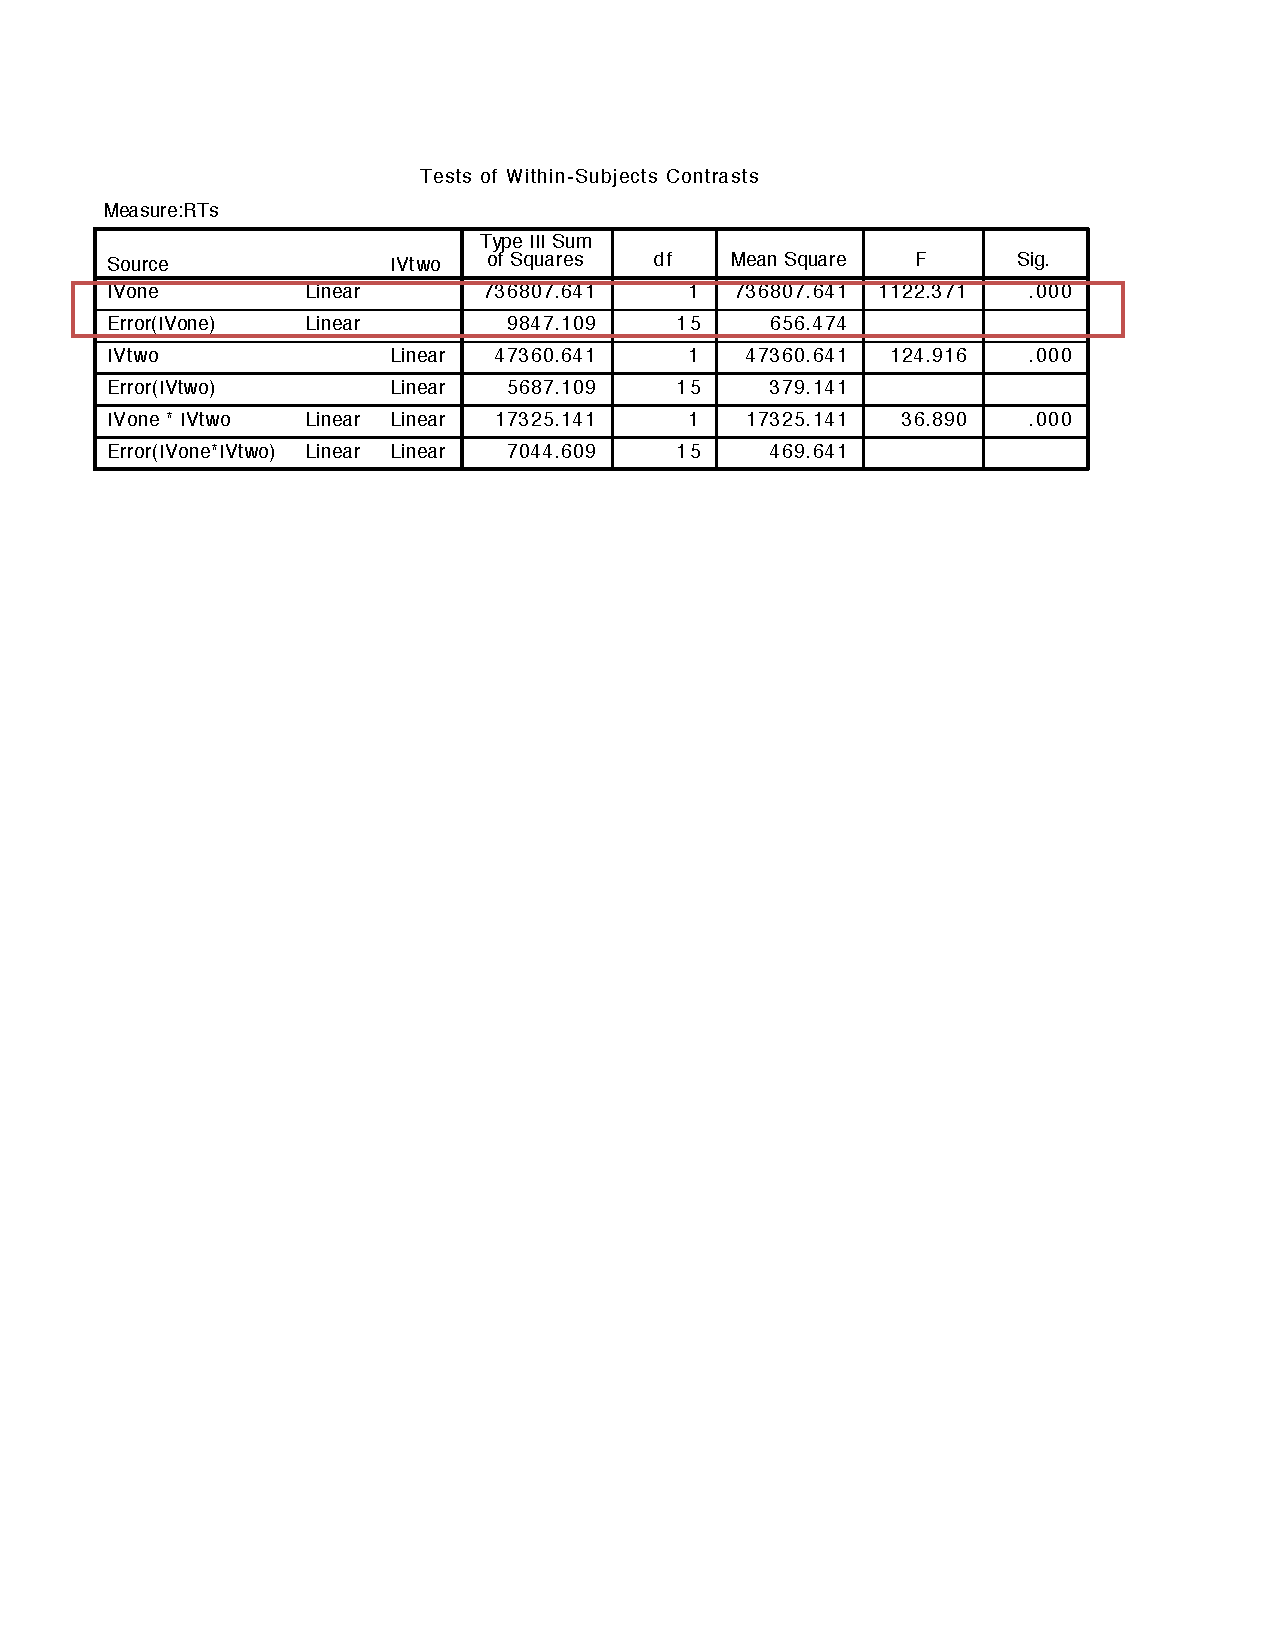
\includegraphics[width=\linewidth]{LabmanualFigures/SPSS13.pdf}
      \caption{ANOVA table}
      \label{fig:SPSS13}
\end{figure}

\subsection{Main effect for IV 1}

Each main effect is listed under source. Each main effect has a corresponding error term listed below. The source for the main effect of independent variable 1 is labeled IV one. You will see it has a corresponding df of 1, an F-value of 112.371, and a p-value <.05. This main effect is significant. You would report this in the following way.

The main effect for independent variable 1 was significant, F(1,15) = 112.371, MSE = 656.47, p<.05. 

The 15 comes from the df from the error term for IVone. As well, the MSE (656.47) comes from the Mean Square from the error term. When you report the main effect, you will also need to report the pattern. The above sentence simply tells the reader that there was a significant difference between the levels of IVone, however it does not explain whether level 1 was larger or smaller than level 2. To report the main effect you will need to compute the averages for each level of IVone. You can do this directly in excel, or you can have SPSS compute these numbers for you by checking the appropriate options before running the analysis. You will need all of the numbers from the above descriptive statistics table. 

First, we find the average for level 1 of IVone (477.5 + 499)/2 = 488

Second, we find the average for level 2 of IVone (659.1875 + 746.5)/2 = 703

Now we can write a complete description of the main effect for IVone. 

The main effect for independent variable 1 was significant, F(1,15) = 112.371, MSE = 656.47, p<.05. Mean performance was lower for level 1 (488) than level 2 (703). 


\subsection{Main effect for IV 2}

Following the same steps as above we look for IV two in the source table and find the dfs, the F-value, the MSE for the error term, and the p-value. 

The main effect for independent variable 2 was significant, F(1,15) = 124.92, MSE = 379.14, p<.05. Mean performance was lower for level 1 (568) than level 2 (623).

\subsection{The interaction effect}

Reporting the interaction uses the same information that you would use to report the main effect. The interaction is listed in the source table as IVone*IVtwo. It has corresponding dfs, F-value, MSE for the error term, and a p-value. 

The interaction between independent variable one and two was significant, F(1,15) = 36.89, MSE = 469.64, p<.05. The difference between level one and level two for independent variable two was smaller for level one (499 - 478 = 21) than level two (747 - 659 = 88) of independent variable 1. 

\subsection{Post Hoc Tests to interpret the interaction}

Post hoc tests are used to clarify the nature of the interaction. In the above example we found a significant interaction. The difference between level 1 and level 2 for IV two was 21 and 88 for level 1 and level 2 of the first independent variable. The significant interaction tells us that 21 and 88 are significantly different from each other. However, we still do not know whether each comparison is significant in an of itself. For example it may be the case that the difference between level 1 and level 2 for IV 2 was only significant for the 2nd level of IV1 (88), and not significant for the 1st level of IV1 (21). In this example you can run a paired t-test, or a one-way repeated measures ANOVA on the specific comparison that you are interested in. For example, you would compare the means from IV1L1/IV2L1 and IV1L1/IV2L2. This comparison would test whether the difference of 21 that was found was actually significant from 0. You will report the statistics for the post-hoc tests in the same manner as you would report t-tests, or F-statistics from the above examples. 